% 编译使用xelatex
\documentclass{ctexart}

\usepackage{amsmath}
\usepackage{amsfonts}
\usepackage{amssymb}
\usepackage{graphicx}
\usepackage{subfigure}
\usepackage{tabularx}

\DeclareMathOperator{\Zset}{\mathbb{Z}}

% for simulating booktabs rules; so they work with vertical lines
\newlength{\Oldarrayrulewidth}
\newcommand{\Cline}[2]{
  \noalign{\global\setlength{\Oldarrayrulewidth}{\arrayrulewidth}}
  \noalign{\global\setlength{\arrayrulewidth}{#1}}\cline{#2}
  \noalign{\global\setlength{\arrayrulewidth}{\Oldarrayrulewidth}}}
\newcommand{\Hline}[1]{
  \noalign{\global\setlength{\Oldarrayrulewidth}{\arrayrulewidth}}
  \noalign{\global\setlength{\arrayrulewidth}{#1}}\hline
  \noalign{\global\setlength{\arrayrulewidth}{\Oldarrayrulewidth}}}
\newcommand{\Topline}{\Hline{0.08em}}
\newcommand{\Bottomline}{\Hline{0.08em}}
\newcommand{\Midline}{\Hline{0.05em}}
\newcommand{\CMidLine}[1]{\Cline{0.05em}{#1}}

% for formatting a row
\newcolumntype{+}{>{\global\let\currentrowstyle\relax}}
\newcolumntype{^}{>{\currentrowstyle}}
\newcommand{\rowstyle}[1]{\gdef\currentrowstyle{#1}#1\ignorespaces}

% define new stretchable column types
\newcolumntype{L}{>{\raggedright\arraybackslash}X}
\newcolumntype{R}{>{\raggedleft\arraybackslash}X}
\newcolumntype{C}{>{\centering\arraybackslash}X}

\addtolength{\oddsidemargin}{-.875in}
\addtolength{\evensidemargin}{-.875in}
\addtolength{\textwidth}{2.00in}
\addtolength{\topmargin}{-.875in}
\addtolength{\textheight}{1.75in}

\title{计算机网络安全技术}

\begin{document}
\maketitle

\tableofcontents

\section{基本密码学}
\subsection{基本概念}
\paragraph{传统加密和私钥加密} 传统加密包含代换, 置换密码及其组合, 重点依赖于算法的保密.
    私钥加密亦称非对称加密, 算法和公约公开, 私钥保密.
\paragraph{块加密和流加密} 输入是字符, 每次是处理一个字符还是处理一组字符.
\paragraph{无条件安全和计算安全} 无条件安全即, 拥有无论多少密文对破译都没有帮助.
    计算安全即, 破译代价大于加密数据本身价值, 或者破译时间长于加密数据有效时间.
\paragraph{记号}
    \begin{description}
        \item[加密函数] $c = E_{K_E}(m),\quad m \in \mathcal{M}, c \in \mathcal{C}, K_E \in \mathcal{K}_E$
        \item[解密函数] $m = D_{K_D}(c),\quad c \in \mathcal{C}, m \in \mathcal{M}, K_D \in \mathcal{K}_D$
    \end{description}

\subsection{代换密码}
    如Caesar密码等单表代换密码, Playfair密码和Vigenere密码等多表代换密码.
\paragraph{攻击} 拥有足够密文即可通过统计学分析破译.

\subsection{置换密码}
    $D(m) = \sigma m$, 要求$\mathcal{M} = \Sigma^L$, $\sigma$是$[0, L)$上的置换.
    代换密码变换的是每个位置上的字母, 而置换密码变换的是消息中各个字母的位置.
\paragraph{攻击} 频率分析, 包括多元组频率分析.

\subsection{对称密码}
\subsubsection{Feistel密码结构}
\paragraph{Feistel的密码观点}
    \begin{enumerate}
        \item 使用乘积密码
        \item 交替使用代换和置换
    \end{enumerate}
\paragraph{Shannon的密码观点}
    \begin{description}
        \item[扩散] 密文不包含明文的统计信息, 每个明文字符影响多个密文字符
        \item[混淆] 复杂的密文和密钥间的统计关系, 防止从密文推出密钥
    \end{description}
\paragraph{Feistel网络}
    大致如图所示.
    \begin{figure}[ht!]
    \centering
    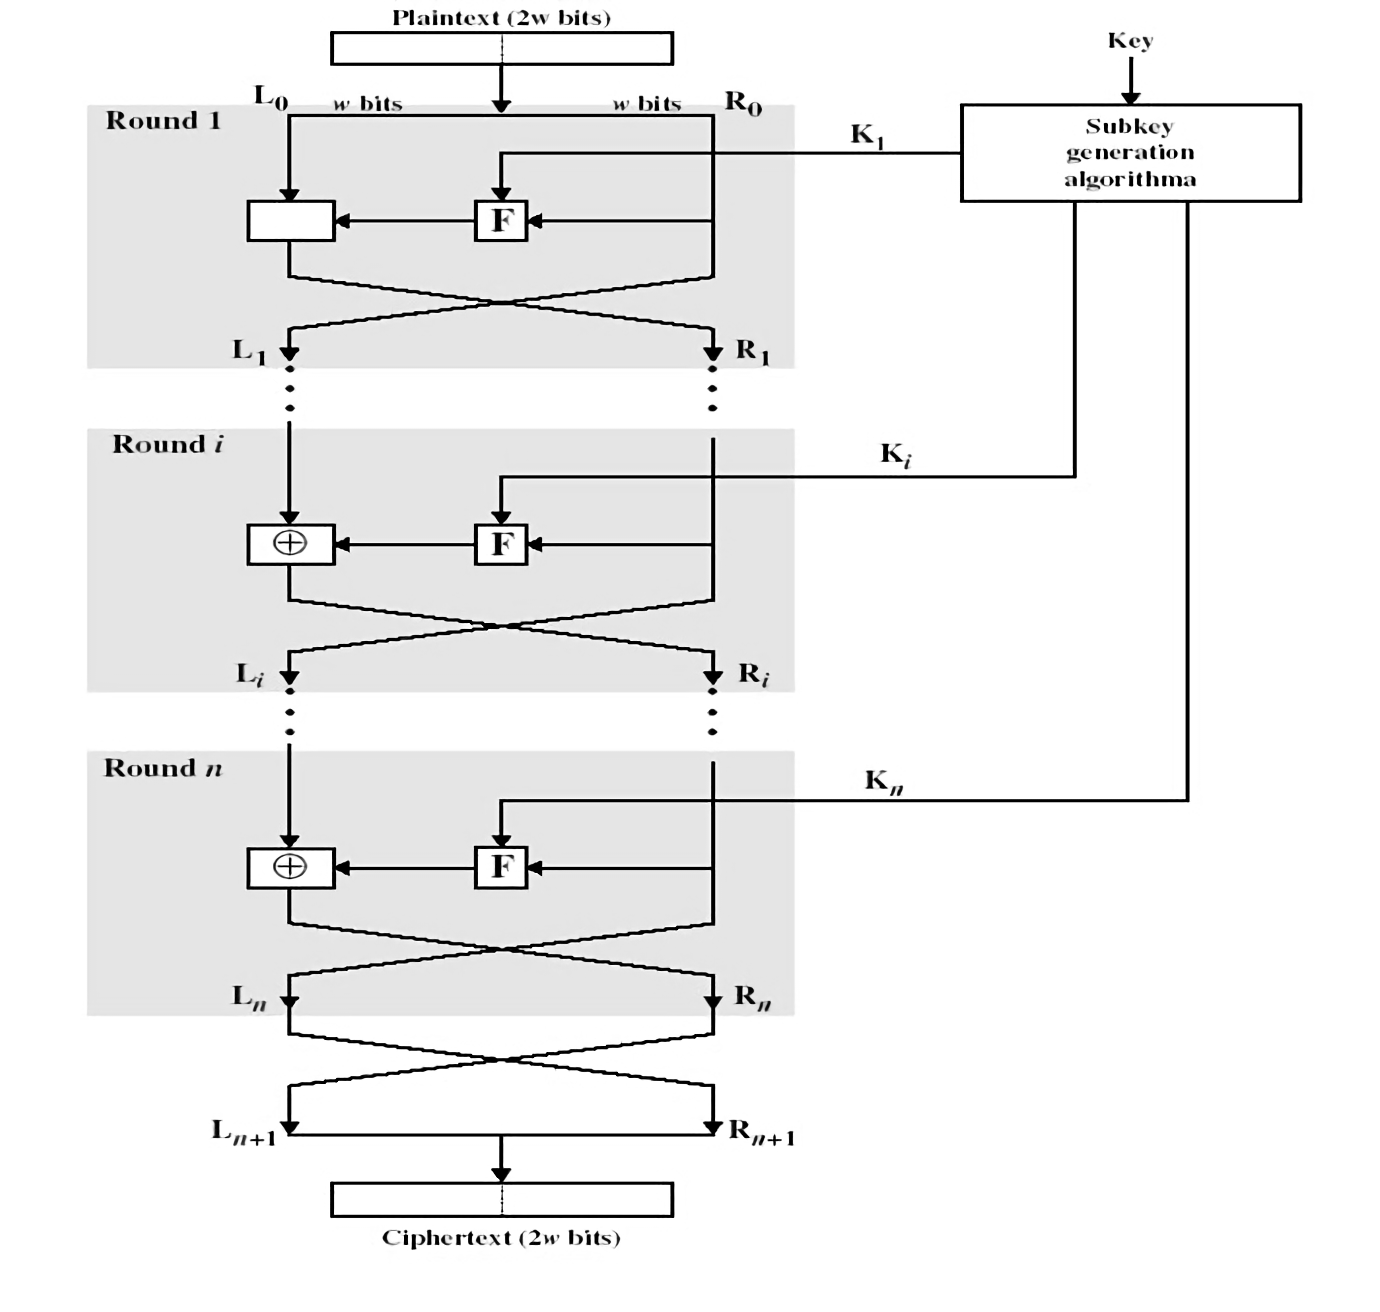
\includegraphics[width=0.6\textwidth]{feistel-net.png}
    \caption{经典的Feistel网络结构}
    \label{lenet-structure}
    \end{figure}
\paragraph{Feistel网络的元素}
    \begin{description}
        \item[分组长度和密钥长度] 越长越安全, 但是效率越低
        \item[迭代层数] 越多越安全
        \item[$K_i$的产生算法] 越复杂越安全
        \item[$F$函数] 越复杂越安全
    \end{description}

\subsubsection{常见对称密码}
    对称密码的特点是只有一个密钥, 加密过程和解密过程是基本相同的.\par
    通信双方如果需要交换密钥, 则需要在安全的信道上交换密钥.\par
    对称密码的速度通常较非对称密码快, 因此常用于大量数据的加密上.\par
\paragraph{DES算法}
    DES是对称密钥算法, 基于Feistel网络结构.
    密钥长度为56位, 块长度是64位, 迭代16轮.\par
    和Feistel的区别是, 加密初始和末尾有一个置换.\par
    已被破解.
\paragraph{3-DES算法}
    密钥长度加倍到112位, 并且加密函数变成了 \[
        \mathbf{3-DES}(M) = \mathbf{DES}(\mathbf{DES}(\mathbf{DES}(M))) \]
    很安全, 但是效率很低.
\paragraph{Blowfish算法}
    基于Feistel网络结构, 但是每轮中左右两半都进行计算.\par
    未被破解.
\paragraph{RC5算法}
    仍然是多轮加密, 但是每轮结构更加复杂.
\paragraph{AES算法}
    AES不是Feistel结构, 每一轮处理整个输入 (而非分成2部分).

\subsubsection{S-DES算法}
    此处的 S-DES 意为 Simplified DES, 主要做教学展示用.
    S-DES基于 Feistel 结构, 输入输出是8位的, 密钥是10位的, 位指二进制位.\par
\paragraph{生成密钥}
    参考图\ref{s-des-keygen}. 其中置换如
    \begin{center}
    \begin{tabularx}{0.8\textwidth}{cCCCCCCCCCC}
    \Topline
    $n$ & $0$  & $1$  & $2$  & $3$  & $4$  & $5$  & $6$  & $7$  & $8$  & $9$ \\
        \Midline
        $P10(n)$ & $2$&   $4$&    $1$&  $6$&   $3$&   $9$&    $0$&   $8$&   $7$&   $5$\\
        $shift_1(n)$ & $1$  & $2$  & $3$  & $4$ & $0$ & $6$  & $7$  & $8$  & $9$ & $5$\\
        $shift_2(n)$ & $2$  & $3$  & $4$ & $0$ & $1$ & $7$  & $8$  & $9$ & $5$ & $6$\\
    \Bottomline
    \end{tabularx}
    \end{center}
    另外函数$P8(0,\ldots 9) = \left\langle 5, 2, 6, 3, 7, 4, 9, 8 \right\rangle$

    \begin{figure}[ht!]
        \centering
        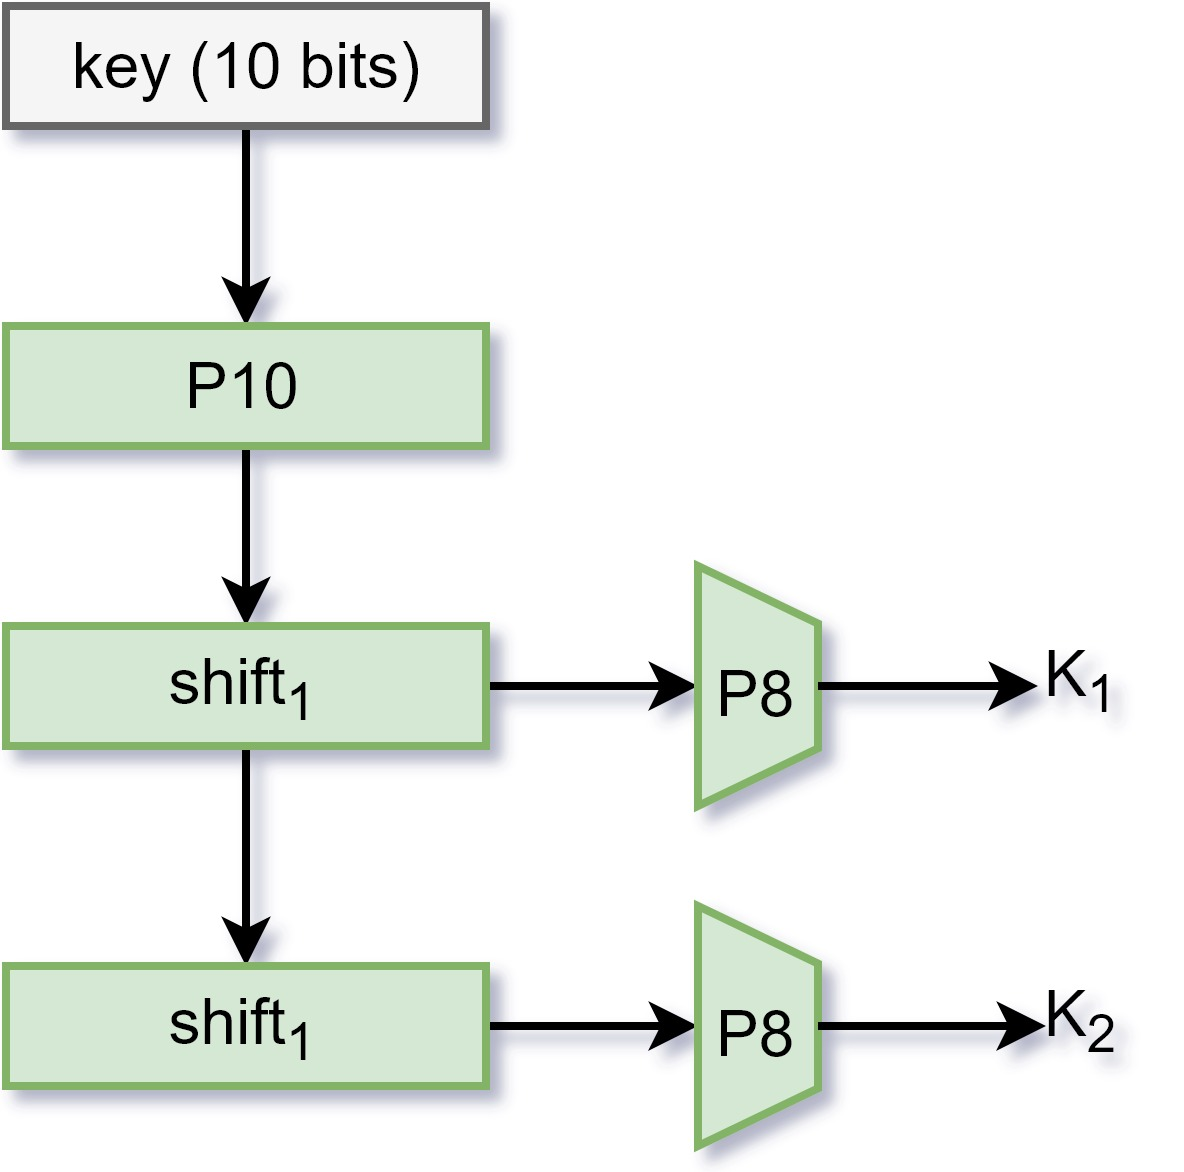
\includegraphics[keepaspectratio,height=0.25\textheight,width=1.0\textwidth]{s-des-keygen.jpg}
        \caption{S-DES 生成密钥}
        \label{s-des-keygen}
    \end{figure}

\paragraph{加密}
    参考图\ref{s-des-enc} 和 \ref{s-des-fk}, 其中有\par
    \[IP(0,\ldots 7) = \left\langle 1, 5, 2, 0, 3, 7, 4, 6 \right\rangle\]
    \[IP^{-1}(0,\ldots7) = \left\langle 3, 0, 2, 4, 6, 1, 7, 5\right\rangle\]
    \[E/P(0, 1, 2, 3) = \left\langle 3, 0, 1, 2, 1, 2, 3, 0 \right\rangle\]
    另外$S$的求法是, $S(n_0, n_1, n_2, n_3)$中, $n_0*2 + n_3$作为行, $n_1*2+n_2$作为列, 寻找矩阵中对应元素\[
        S_0 = \begin{bmatrix}
            01 & 00 & 11 & 10\\
            11 & 10 & 01 & 00\\
            00 & 10 & 01 & 11\\
            11 & 01 & 11 & 10\end{bmatrix}\qquad
        S_1 = \begin{bmatrix}
            00 & 01 & 10 & 11\\
            10 & 00 & 01 & 11\\
            11 & 00 & 01 & 00\\
            10 & 01 & 00 & 11\end{bmatrix}
    \]
    \begin{figure}[ht!]
        \centering
        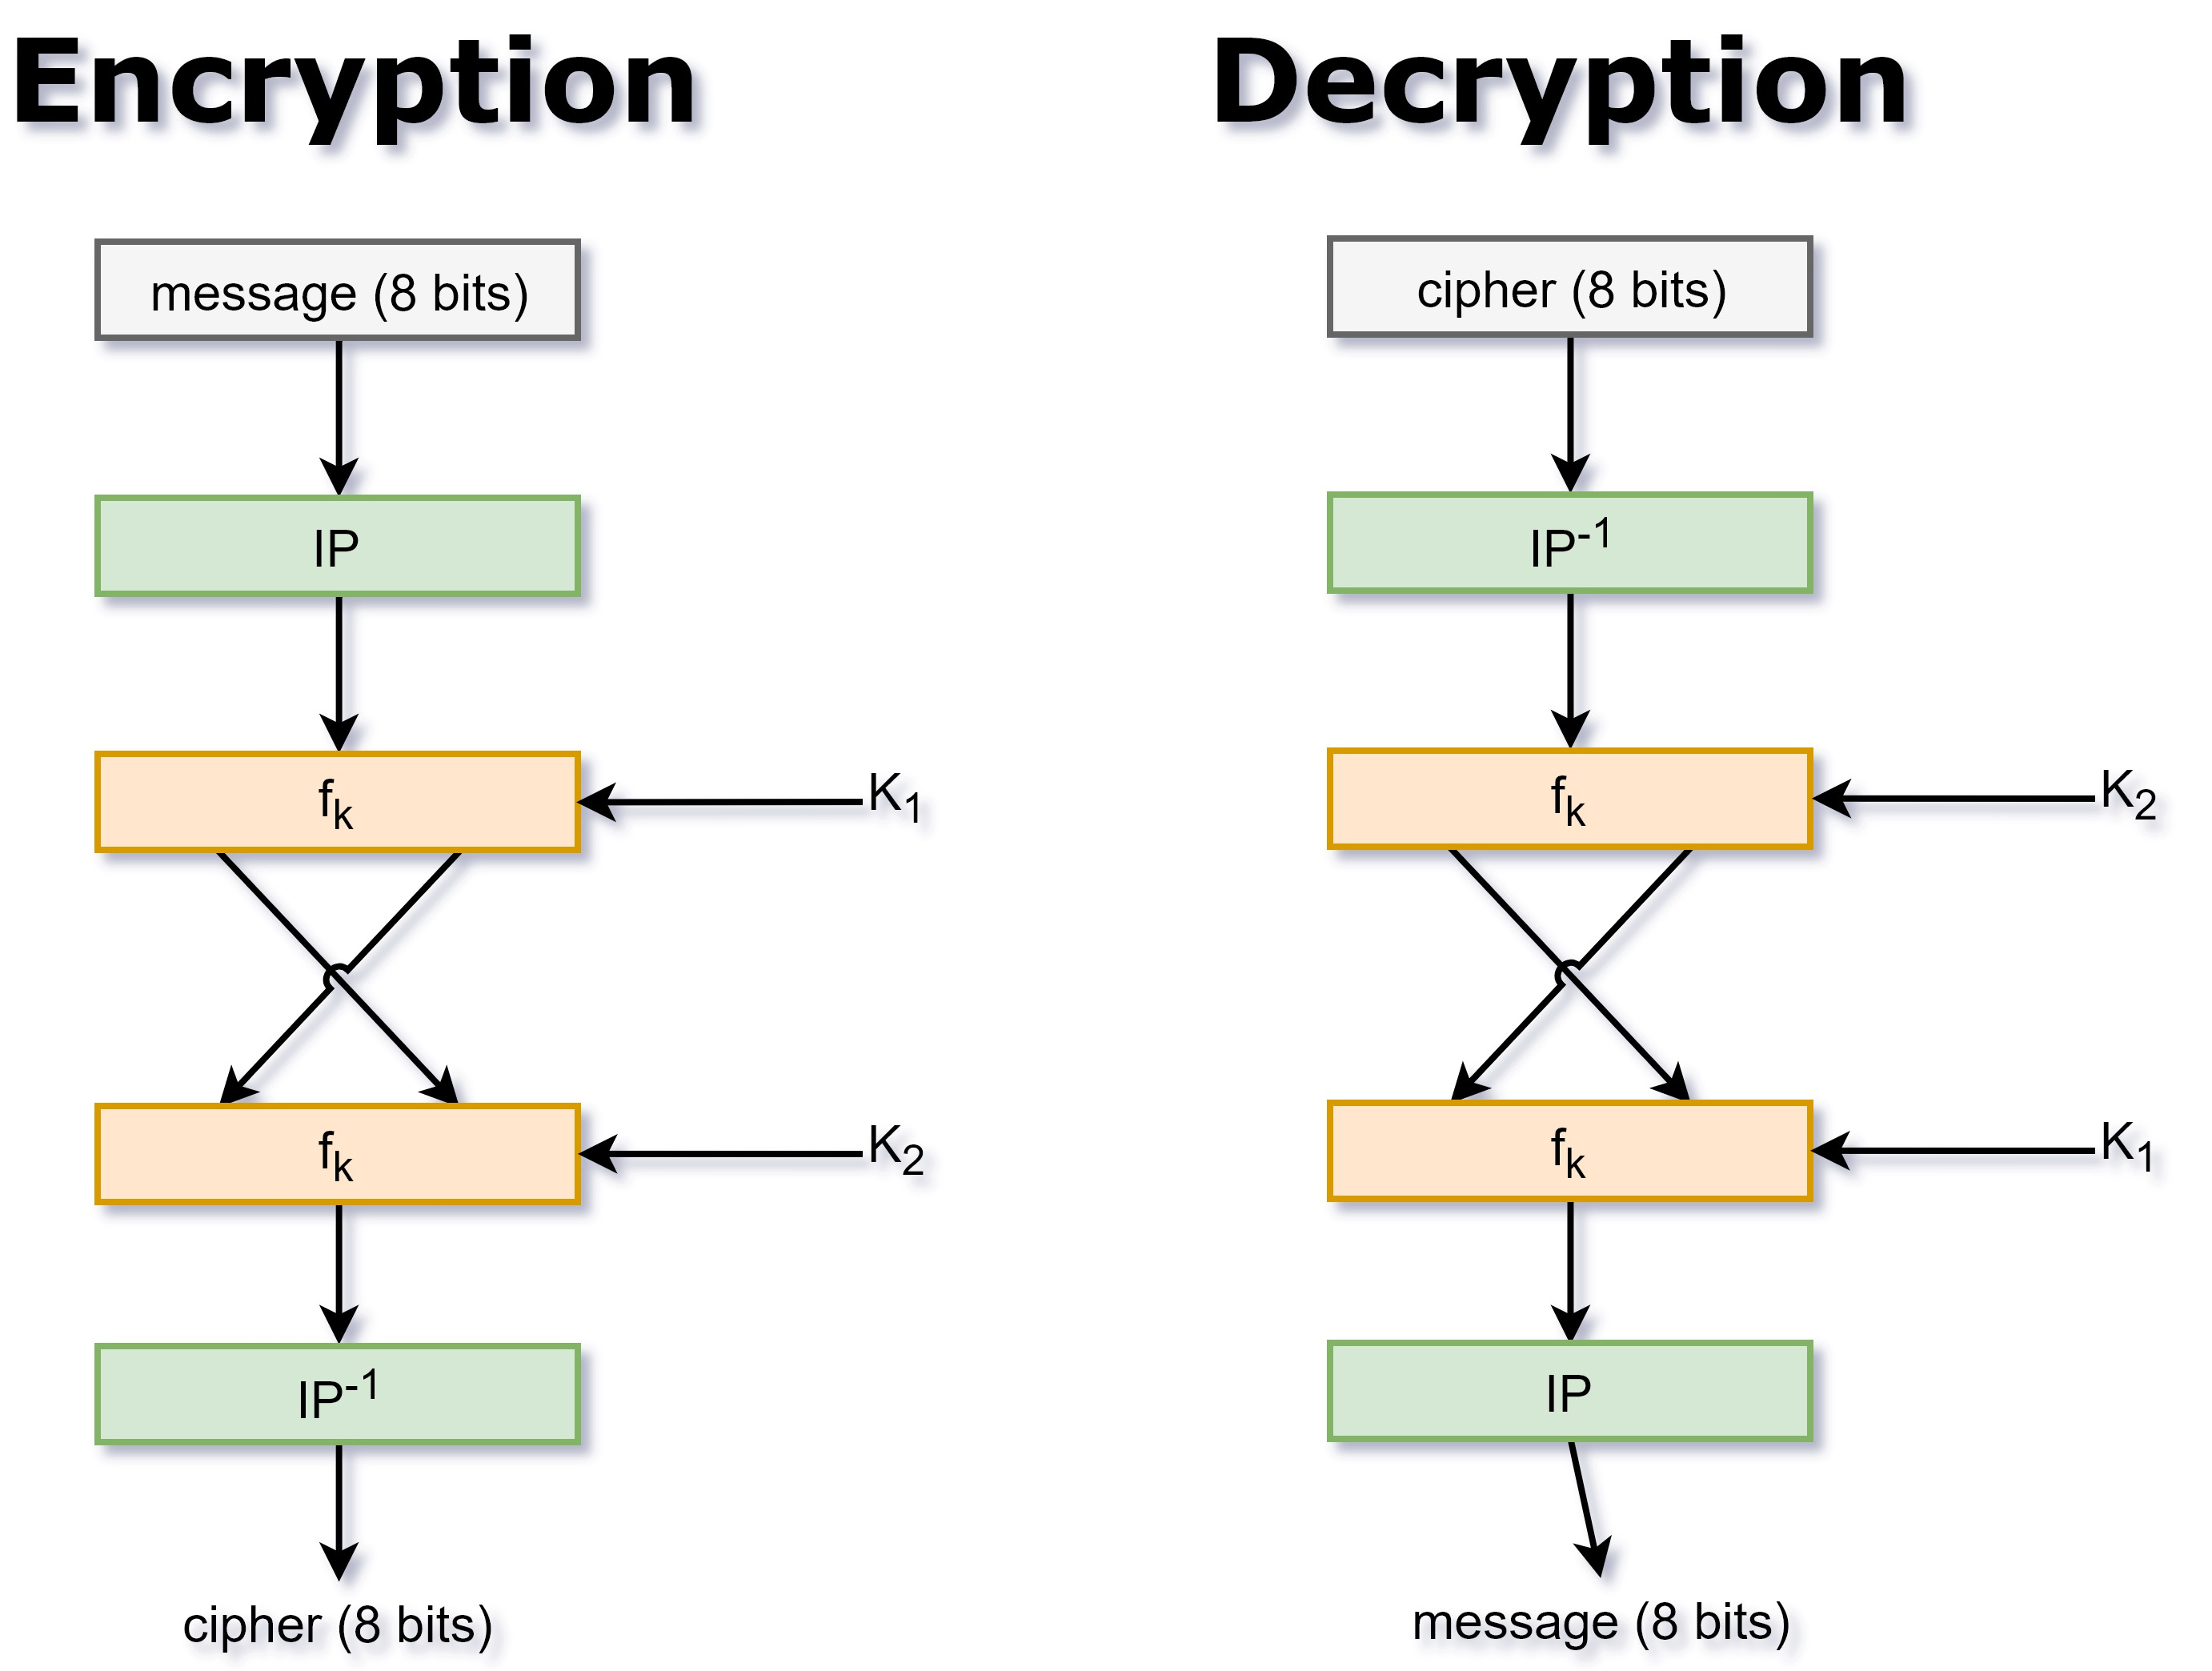
\includegraphics[height=0.5\textheight,width=0.8\textwidth,keepaspectratio]{s-des-enc.jpg}
        \caption{S-DES 加密}
        \label{s-des-enc}
    \end{figure}

    \begin{figure}[ht!]
        \centering
        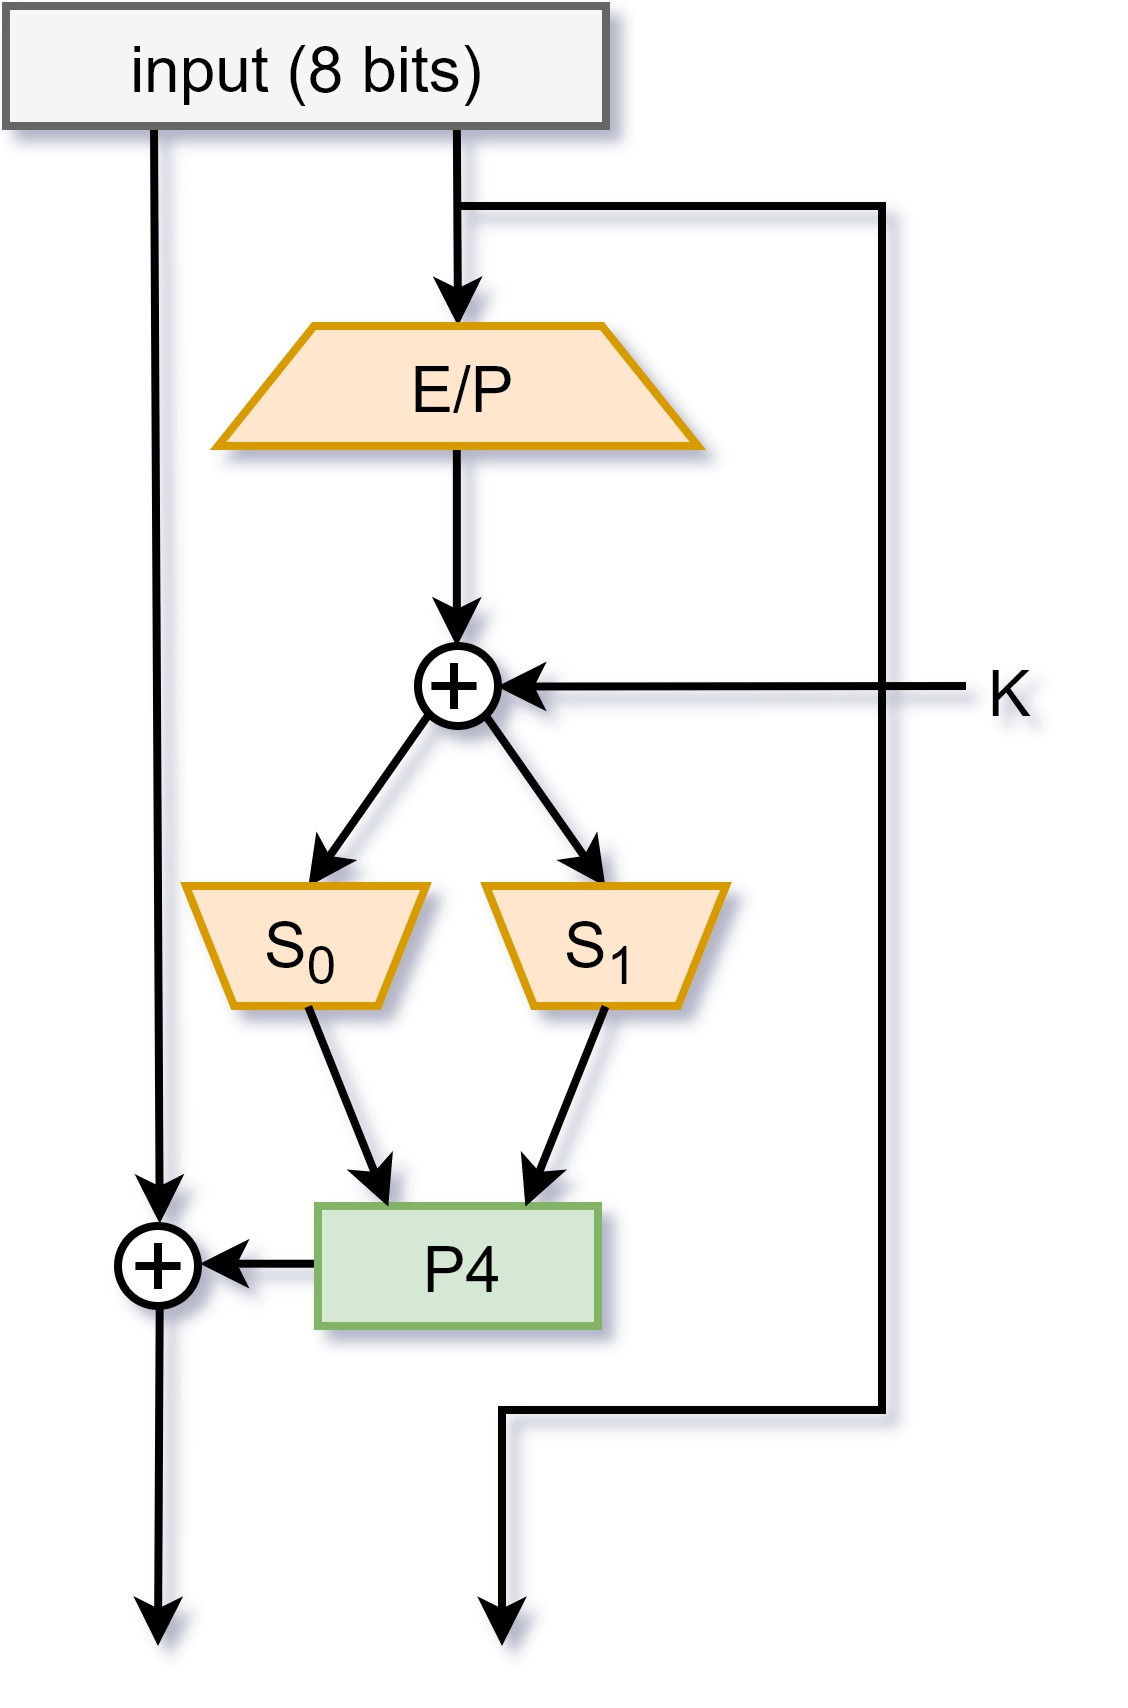
\includegraphics[height=0.5\textheight,width=0.5\textwidth,keepaspectratio]{s-des-fk.jpg}
        \caption{S-DES 的 $F$函数}
        \label{s-des-fk}
    \end{figure}

\subsection{公钥密码}
    公钥密码即非对称密码.
    其中加密和解密使用的是不同的密钥, 称为公钥和私钥.
    \emph{公钥公开, 用于加密和验证签名; 私钥保密, 用于解密和签名.}\par
    非对称密码的速度通常较对称密码要慢,
    所以常常只用于签名\footnote{验证发送者身份的过程},
    或者用于加密发送对称密码的密钥.
\paragraph{加密方法} Alice 向 Bob 发送希望加密的信息, 则 Alice 使用 Bob 的公钥加密信息后发送给 Bob.
\paragraph{签名算法} Bob 希望验证 Alice 的身份,
    其给出一个特定的消息, 要求 Alice 用 Alice 自己的私钥加密后发送给 Bob,
    之后 Bob 再用 Alice 的公钥解密验证.
\subsubsection{RSA算法}
    原文和密文都是$[0, N)$中的整数, 常常$N$是2的幂.\par
\paragraph{前置}
    \begin{enumerate}
        \item 计算大素数 $p$, $q$.
        \item 计算$N = pq$, 公开.
        \item 寻找一个小整数$e,\;e < N,\,(e, N) = 1$
        \item 求解$d e \equiv 1 \pmod{\varphi(N) = (p-1)(q-1)}$, 得到$d$
        \item 公钥为$\langle e, N \rangle$, 私钥为$\langle d, N \rangle$
    \end{enumerate}
\paragraph{加密}
    对于$m \in [0, N)$, 加密函数如下
    \[ E(t) = m^e \bmod N \]
\paragraph{解密}
    对于$c \in [0, N)$, 加密函数如下
    \[ D(c) = c^d \bmod N \]
\paragraph{原理}
    有效性由Euler定理保证 \[ a^{\varphi(n)} \equiv 1 \pmod{n},\quad \forall a\,:\,(a, n) = 1 \]
    安全性由大数分解困难性保证.
\paragraph{攻击}
    \begin{description}
        \item[暴力破解] 需要枚举$t \in [0, N)$的空间
        \item[数学攻击] 因子分解$N$
        \item[计时攻击] 按照加密时间推测私钥.
    \end{description}
\subsubsection{Diffie-Hellman算法}
    用于密钥交换, 而非加密解密, 即通过双方自身的私有密文得到一个共有密文.
\paragraph{前置}
    \begin{enumerate}
        \item 寻找素数$p$, 以及$\Zset_p$的生成元$a$ i.e. $a$是原根, 均公开.
    \end{enumerate}
\paragraph{私有密文产生共有密文}
    \begin{enumerate}
        \item 双方由自己的私有密文$X_A,\, X_B$计算公开的$Y_A = a^{X_A} \bmod p,\, Y_B = a^{X_B} \bmod p$
        \item 双方由公开的$Y_A, Y_B$计算得到共有密文$K = Y_B^{X_A} \bmod p = Y_A^{X_B} \bmod p = a^{X_A X_B} \bmod p$
    \end{enumerate}
\paragraph{原理}
    安全性由离散对数困难性保证.
\subsubsection{和对称密码的比较}
    \begin{itemize}
        \item 笼统地说, 非对称密码并不比对称密码安全.
        \item 非对称密码不是通用的, 对称密码仍然由于快速而广泛使用
        \item 公钥密码的密码分配不必传统密码分配简单
    \end{itemize}

\subsection{密钥分配}
\subsubsection{传统对称密钥分配}
\paragraph{可能的方法}
    \begin{enumerate}
        \item Alice选择密钥, 亲自交给Bob
        \item 第三方Charlie选择密钥, 亲自交给Alice和Bob
        \item Alice选择密钥, 用最近使用的密钥加密后发给Bob
        \item 第三方Charlie选择密钥, 通过某个秘密渠道交给Alice和Bob
    \end{enumerate}
\paragraph{密钥分发中心}
    基本假设: 每个人有一个仅他自己和KDC知道的主密钥. 此假设下, Alice和Bob得到一次性次密钥的方法为:
    \begin{enumerate}
        \item Alice向KDC请求次密钥
        \item KDC发送给Alice消息, 消息用$PK_a$加密, 包含用次密钥$K_s$, 以及$PK_b$加密的$K_s$和$ID_a$
        \item Alice将$PK_b$加密的消息发送给Bob
    \end{enumerate}
    为了效率和安全性, KDC通常也是层次性的, 而非一个巨大的中心KDC.
\subsubsection{非对称公钥发布}
\paragraph{公开发布} Alice向所有人广播自己的公钥. 问题是容易伪造广播消息.
\paragraph{公开目录} 只有一个受信任的实体 (管理员) 能够广播公钥. 问题是如果受信任的实体被攻击, 公钥可以任意更改.
\paragraph{公钥授权} 双方通讯之前先向管理员请求对方公钥, 管理员返回消息时用管理员私钥加密.
\subsubsection{通过非对称公钥分配传统密钥}
    非对称加密的问题是效率太低, 一般通过非对称加密传输传统密钥, 之后消息用传统加密方法求解.
\paragraph{Merkel朴素方法} Alice给Bob请求共有密钥. Bob用Alice公钥加密某密文后传输给Alice, Alice之后使用自己的私钥解密得到共有密文.
    问题: 中间人攻击, 考虑若Bob是假Bob.
\paragraph{保密真实方法} \begin{enumerate}
        \item Alice发送给Bob: $E_{K_{B, pub}}(ID_A, N_A)$, $N_A$是一个随机校验数
        \item Bob得到$ID_A, N_A$, 发送给Alice: $E_{K_{A, pub}}(N_A, N_B)$
        \item Alice得到$N_A', N_B$, 检查$N_A = N_A'$, 发送给B$E_{K_{B, pub}}(N_B)$
        \item Bob得到$N_B'$, 检查$N_B = n_B'$
    \end{enumerate}


\section{计算机网络安全体系结构}
\subsection{安全目标}
    \begin{description}
        \item[保密性 Confidentiality] 未授权的实体不能获得信息内容
        \item[完整性 Integrity] 信息不能被篡改, 或者能检测篡改
        \item[可用性 Availability] 授权用户能够访问资源, 防止DoS攻击
    \end{description}
\subsection{手段}
    \begin{description}
        \item[加密] 防止未授权的外人获得通信内容, 如防止窃听.
        \item[认证] 验证通信对等体的身份真实性, 如防止中间人攻击. 可以通俗的理解为, ``发送这条消息的人的确是 Alice''.
        \item[数字签名] 相当于对通信对等体和消息同时认证, 如防止抵赖. 可以通俗的理解为, ``Alice 的确发送过这条消息''.
    \end{description}

\section{消息认证}
\subsection{攻击类型}
    \begin{description}
        \item[泄密] 保密性范畴.
        \item[传输分析] 保密性范畴.
        \item[伪装] 消息认证.
        \item[内容修改] 消息认证.
        \item[抵赖] 数字签名, 以及协议设计.
    \end{description}
\subsection{消息认证基本概念}
\subsubsection{消息认证} 确认发送方是真实的, 确认消息违背篡改.
    \begin{quote}{\itshape 消息认证就是验证所收到的消息确实是来自真正的发送方且未被修改的消息}\end{quote}
\subsubsection{基本框架} 发送方产生一个认证符; 接收方产生一个认证符, 并且检查双方认证符是否匹配.

\subsection{产生认证符}
\subsubsection{消息加密作为认证符}
\paragraph{对称加密} 为了认证, 要么消息空间是稀疏的, 要么消息中带有校验符号 FCS.
    FCS 的计算是在加密之前, 将发送的内容计算出一个校验符, 附到发送内容后一并加密发送.\par
    可以提供加密和认证, 但是无法提供数字签名.
\paragraph{非对称加密} 使用私钥加密可以完成签名和认证, 使用公钥加密可以提供保密性,
    两者都使用可以同时提供加密和认证以及签名.\par
    但是这样需要 4 次加解密运算, 代价较高.
\subsubsection{消息认证码MAC}
    通过消息和密钥 (两者都需要, 以验证\emph{这条消息}是发自这个\emph{发送者}),
    利用公开的算法计算消息认证码 $MAC = C_K(M)$,
    其中$K$是共有密钥, $M$是消息, $C_K$生成一个固定长度的短数据块.\par
    提供认证, 但是不提供数字签名: 接收方也有$K$, 因此可以伪造消息.\par
    可以先加密在使用MAC, 提供加密和认证.
\subsubsection{消息哈希}
    通过消息, 计算认证符 $MD = \mathbf{Hash}(M)$, $M$是消息, $\mathbf{Hash}$输出固定长度的短数据. 亦称消息摘要.\par
    哈希本身不包含对于发送者的验证, 因此一定要对哈希加密. 根据需要的服务, 具体有\begin{itemize}
        \item 对称加密中, 可以加密消息和哈希码, 可以完成加密和认证.
        \item 对称加密中, 可以只加密哈希码, 可以完成认证.
        \item 非对称加密中, 用发送方的私钥加密哈希码, 可以完成认证和数字签名.
        \item 非对称加密中, 用发送方的私钥加密消息和哈希码, 可以完成加密, 认证和数字签名.
    \end{itemize}

\subsection{哈希函数}
\subsubsection{哈希函数的理论要求}
    要求哈希函数$h = H(M)$有如下性质 \begin{description}
        \item[单向性] 对于$h$, 难以寻找$M$, 满足$H(M) = h$
        \item[弱抗碰撞] 对于$M$, 难以寻找$M'$, 满足$H(M) = H(M')$
        \item[强抗碰撞] $\forall M$, 难以寻找$M'$, 满足$H(M) = H(M')$
    \end{description}
\subsubsection{安全哈希函数的Merkel结构}
    参见图 \ref{merkel-hash}.
    \begin{figure}[ht!]
    \centering
    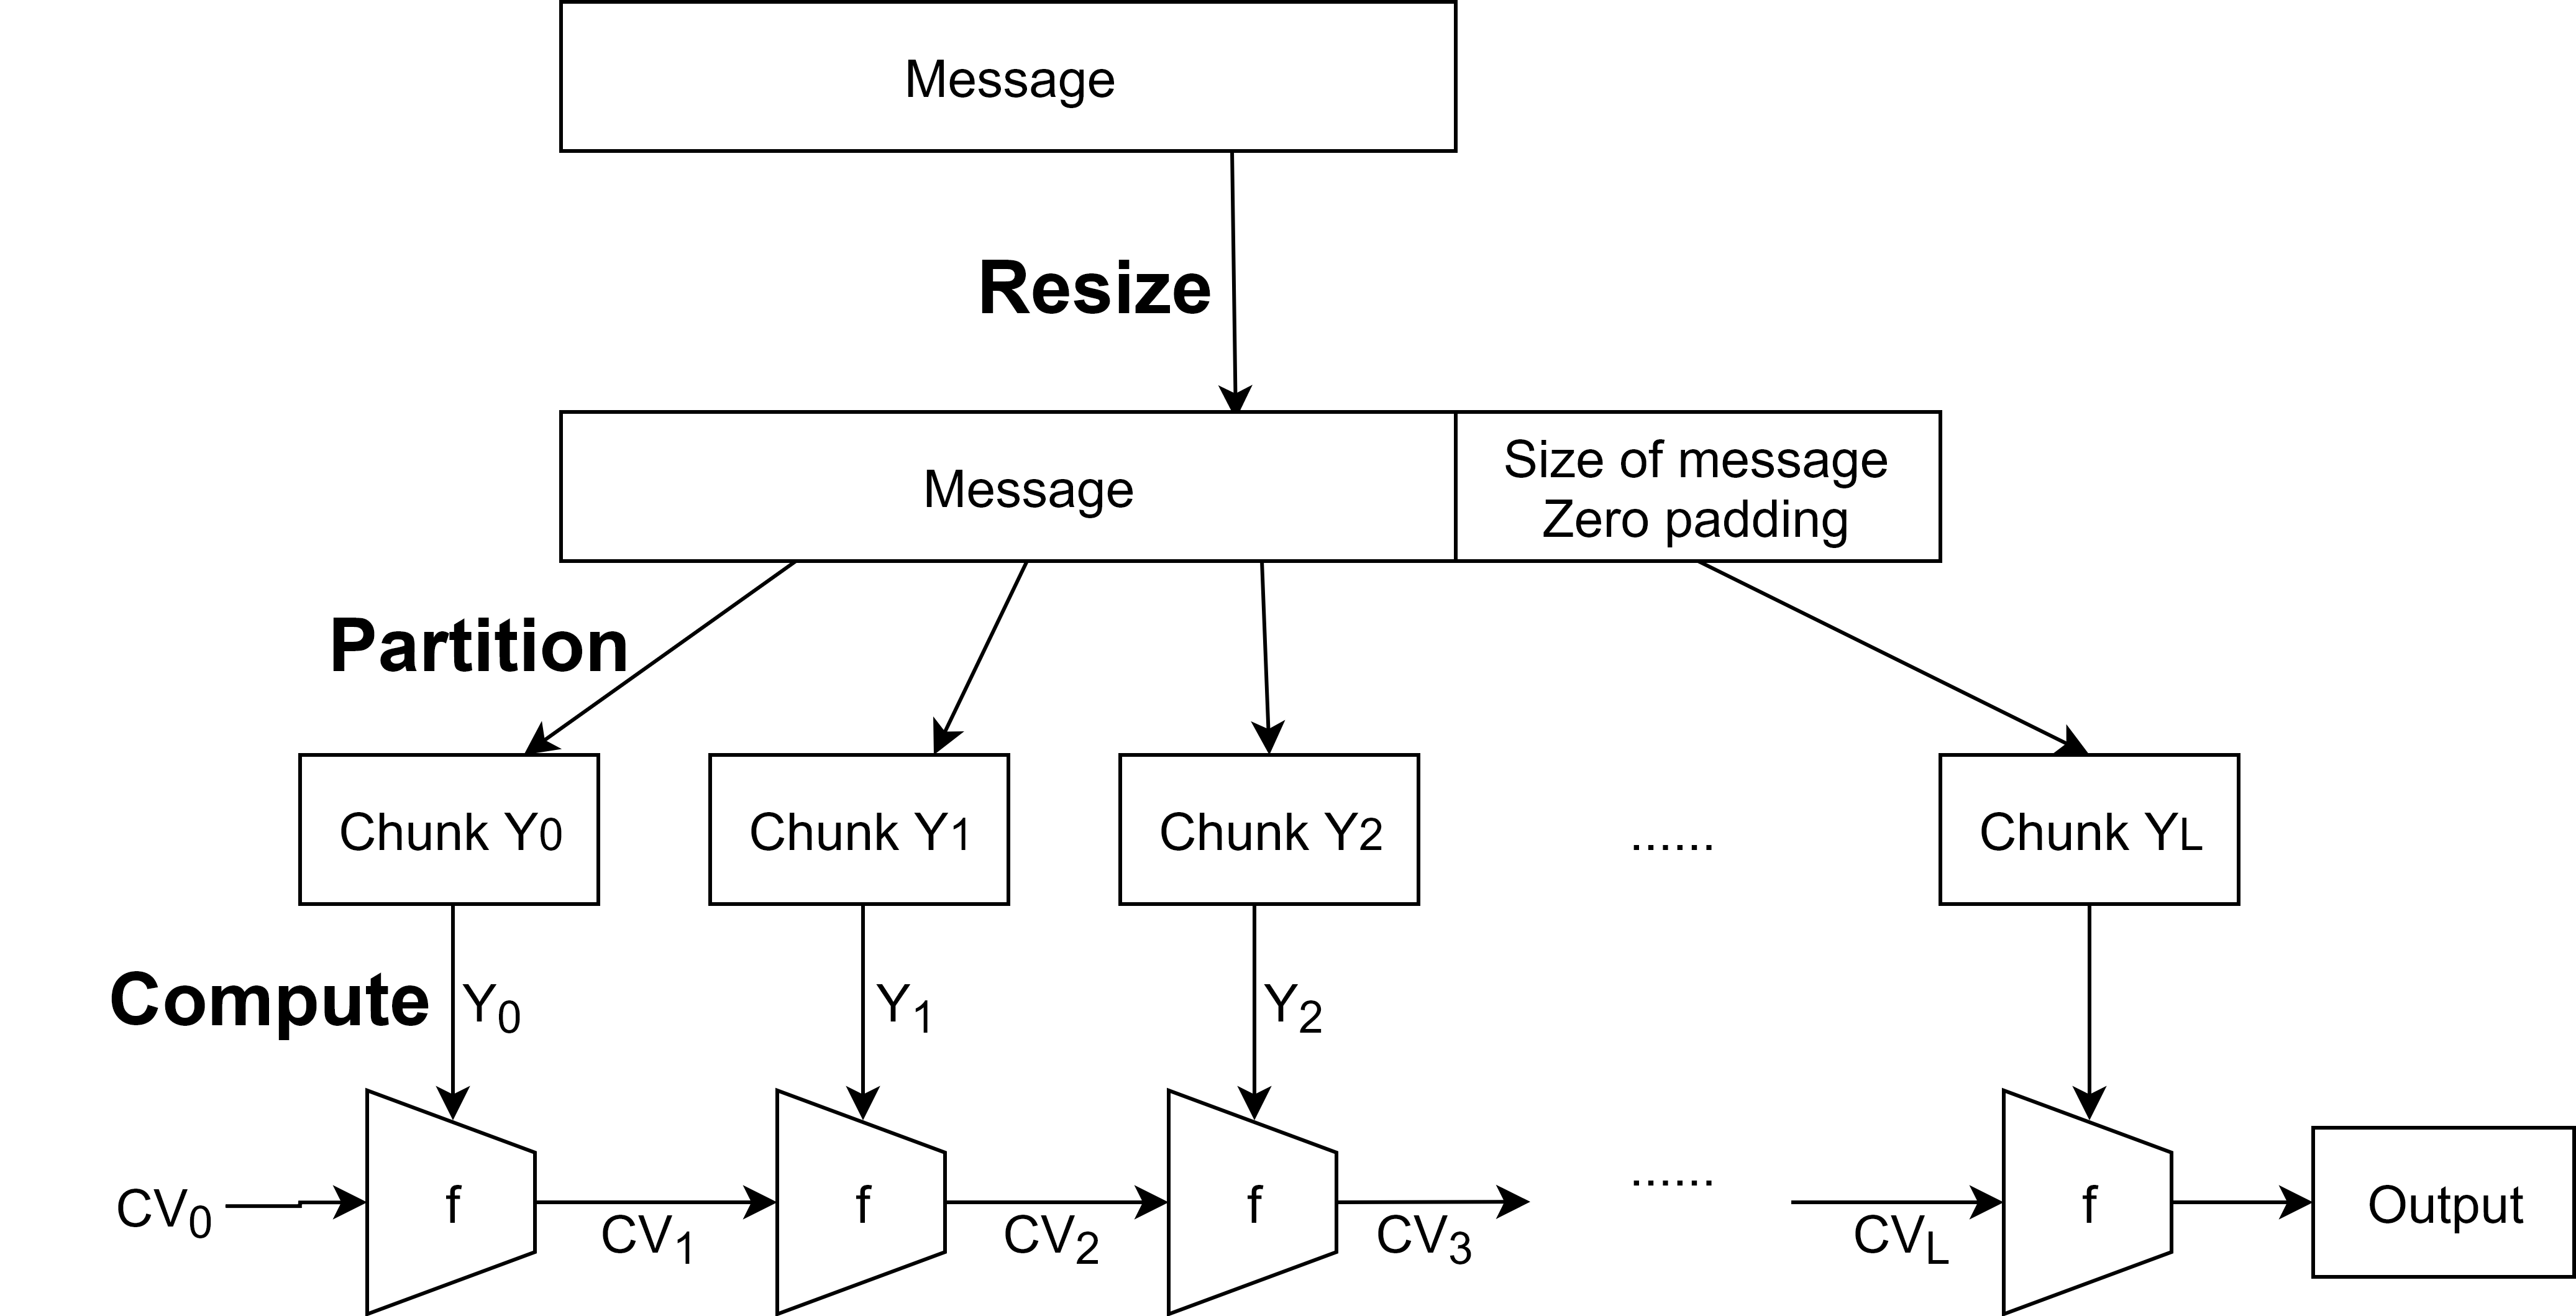
\includegraphics[width=0.8\textwidth]{merkel-hash}
    \caption{Merkel哈希结构}
    \label{merkel-hash}
    \end{figure}
\subsubsection{常用哈希举例} 有MD5, SHA-1, SHA-2, GOST等等.
\paragraph{MD5} 有如下特点 \begin{itemize}
        \item 消息可以无限长
        \item 采用小端结构, 将消息表示为 32 位字的序列
        \item 填充部分包含了消息的长度
        \item 填充后消息位数是 512 的倍数, 每个分组$Y_i$大小为 512 位 (64字节, 16个字)
        \item 中间结果$CV_i$和最后结果$MD$的长度是 128 位 (16字节, 4个字寄存器)
        \item 由四轮运算组成, 每轮16步迭代
    \end{itemize}


\subsection{数字签名DSS算法}
\paragraph{应用场景} 来自消息发送双方的攻击, 如接收方伪造发送, 发送方抵赖发送.
\paragraph{分类} 直接数字签名 (仅通信双方), 仲裁数字签名 (受信任的实体).
\paragraph{前置} \begin{description}
    \item[全局公钥] $p$是素数\\ $q$是素数且$q \mid p -1$\\
        $g = h^{(p-1) / q} \bmod p$
    \item[用户私钥] $x$, 满足$x < q-1$
    \item[用户公钥] $y = g^x \bmod p$
    \item[随机数] $k < q$, 每次认证都应产生一个新的$k$, 且$k$保密
    \end{description}
\paragraph{DSS算法签名} 签名用一组数$(r, s)$代表, 计算过程如下方程, 哈希函数$\mathbf{H}$一般取SHA-1
    \begin{align*}
        r &= g^k \bmod p \bmod q\\
        s &= (k^{-1} (\mathbf{H}(M) + xr)) \bmod q
    \end{align*}验证要求 \begin{equation*}
        g^{(s^{-1} M) \bmod q} y^{(s^{-1} r) \bmod q} = r
    \end{equation*}

\section{访问控制}
\subsection{基本概念}
\paragraph{主体} 提出访问资源请求的人/实体.
\paragraph{客体} 含有被访问资源的实体.
\paragraph{访问} 对资源的使用行为, 有时还需包括主客体.
\paragraph{访问控制矩阵} 定义不同主体对于不同客体可以执行的操作, 如
    \begin{center}
        \begin{tabularx}{0.6\textwidth}{|C|C|C|C|}
            \hline
             & $O_2$ & $O_3$ & $O_4$\\
            \hline
            $S_1$ & R/W & R & \\
            \hline
            $S_2$ & W & & \\
            \hline
            $S_3$ & R/W & R/W & R/W\\
            \hline
        \end{tabularx}
    \end{center}
    按列看, 就是客体的访问控制列表; 按行看, 就是主体的访问能力列表.

\subsection{访问控制模型}
\subsubsection{自主性访问控制}
    每个客体有一个管理者, 管理者将访问权限授权给其他人. 可以看成以主体为核心.
    如Unix文件系统.\par
\paragraph{性质}
    易用方便灵活. 但是不能控制信息的流动, i.e. 其他人取得资源后可以自由分发.
\subsubsection{强制性访问控制}
    每个主体和客体有固定的安全级别, 由系统管理员决定. 可以看成以客体为核心.
\paragraph{No Read Up}
    主体只能读取安全级别更低的客体.
\paragraph{No Write Down}
    主题只能写入安全级别更高的客体.
\subsubsection{基于角色的访问控制}
    主体(用户)属于用户组(角色). 每个角色(而非主体)对于不同的客体有不同访问权限.
    可以看成以访问为核心.

\subsection{防火墙}
    在两个不同网络间建立访问控制的软硬件.
\subsubsection{设计目标}
    监控两个网络间所有通信流量, 只有授权的流量才允许通过.
\subsubsection{常用技术} 基于控制, 有\begin{description}
        \item[服务控制] 基于服务端口号 / IP地址
        \item[方向控制] 内到外 / 外到内
        \item[用户控制] 基于用户的身份, 如 VPN
        \item[行为控制] 基于用户的行为进行控制, 如垃圾邮件过滤
    \end{description}\par
    基于分层, 有\begin{description}
        \item[网络层] 包过滤技术.\\
            根据定义好的过滤规则, 包含IP地址, 端口和协议等, 审查每个数据包. 性能较高, 但控制能力不强.\\
            如路由器中的ACL.
        \item[网络层] 地址转换.\\
            完成转发和地址转换. 不提供额外的安全性,但是可以隐蔽内部网络,节省地址空间
        \item[传输层] 电路层网关.\\
            检查包所属的会话, 即是不是属于客户端和服务器的某一个链接, 不检查协议和内容.
            不支持无连接的UDP, 性能开销较大.
        \item[应用层] 应用层代理.\\
            功能强大, 但是性能较低, 并且实现麻烦.
    \end{description}

\subsubsection{访问控制列表} 一组预先定义好的规则. 其根据包头, 指定包是否被拦截.
\paragraph{标准和拓展} 标准ACL只检查 Frame 中源IP地址.
    拓展ACL还支持端口, 目标IP, 协议, 检查 Frame 和 Packet.\par
    路由过程中, 路由前后分别有入口/出口端ACL. 入口端ACL在查路由表前检查, 出口端ACL在转发前检查.

\subsection{VLAN虚拟局域网}
\paragraph{基本概念} VLAN类似一个独立的网桥, 但是可能一个VLAN跨越不同的交换机, 同一个交换机有不同的VLAN.
\paragraph{类型} 如 \begin{description}
        \item[基于物理接口] 按照交换机的接口分配.\\ 配置简单, 但是不灵活.
        \item[基于MAC地址] 局域网中每个MAC地址有对应的VLAN分组.
        \item[基于协议] 根据网络层协议分划VLAN.
    \end{description}
\paragraph{优点} \begin{itemize}
        \item 解决人员维护性
        \item 控制广播流量, 防止交换机后向学习的洪泛造成的``洪范灾难''
        \item 增强安全性
    \end{itemize}
\paragraph{缺点} 缺乏标准

% \section{网络安全协议}
%     协议基本要素: 层次 (OSI 7层中哪一层), 格式, 行为 (亦称控制).

\section{IP层级安全}
\subsection{IPsec}
    与 IP 在同一层. 功能 \begin{description}
        \item[认证] 确认包的发送者真实, 包不被篡改
        \item[加密] 流量管理
        \item[密钥管理] 密钥的安全交换
    \end{description}
\subsubsection{SA}
\paragraph{背景} 假设 Alice 希望给 Bob 发送数据.
    无论加密 (对称加密) 还是认证 (HMAC\footnote), 他们都需要一个共有的密钥.
    IPsec讨论中假设这个双方已有这个共有密钥了.
\paragraph{SPD} 安全策略数据库, 其过滤所有IP流量.
    并且对于每个IP包, 其指定对于此IP包的处理,
    是丢弃\verb/DISCARD/, 直接通过IP发送\verb/BYPASS/,
    还是通过IPsec\verb/PROTECT/.
    如果指定是\verb/PROTECT/, 它还需指定是\verb/ESP/还是\verb/AH/,
    使用传输模式还是隧道模式,
    之后或者利用IKE生成一个SA记录到SAD中, 或者交由SAD处理.
\paragraph{SA内容} Bob 可能有很多个入境连接都使用 IPsec,
    因此每个连接都需要一个标识, 用来让 Bob 确定这个连接的参数,
    如哈希算法, 公共密钥等. IPsec中此标识实现为 SPI, 是一个 32 位的整数.\par
    Bob本地有一个 SAD, 对于每一个有效的 SPI 在 SAD 中都有对应的SA (包含SPI, 使用ESP还是AH, 目标IP地址),
    以及源地址, SA记录等等.
\paragraph{传输模式和隧道模式}
    对于加密或认证, 如果针对的是IP载荷 (即TCP头加载荷), 则成为传输模式, 用于端到端的传输. 通常就在主机上实现.
    如果针对的整个IP包, 则成为隧道模式, 用于网络上构建VPN. 通常在防火墙或者路由器上实现.
\paragraph{原理} IPsec有两种协议, 有AH, 用于认证; 以及ESP, 用于加密和可选的认证. 参见如图\par
    \begin{figure}[ht!]
    \centering
    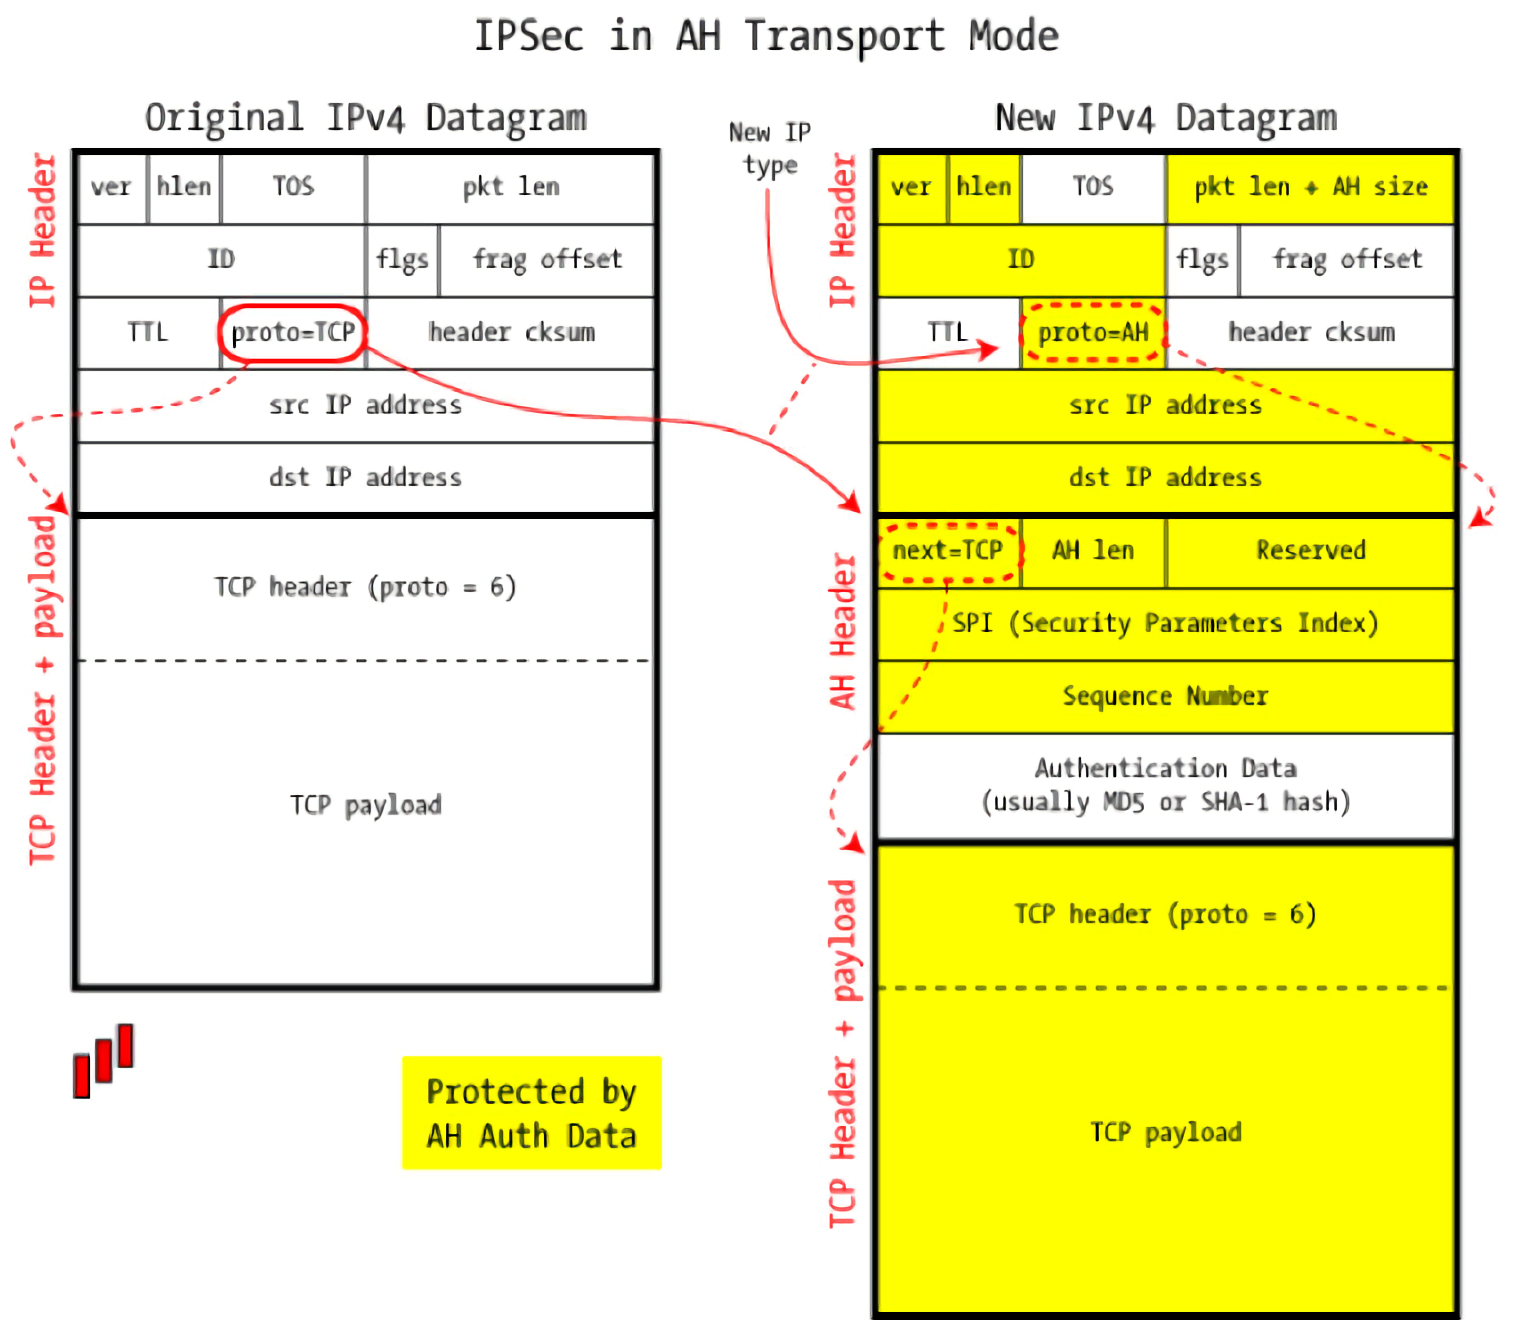
\includegraphics[width=1.0\textwidth]{ah-transport.png}
    \caption{传输模式的AH}
    \label{ah-transport}
    \end{figure}

    \begin{figure}[ht!]
    \centering
    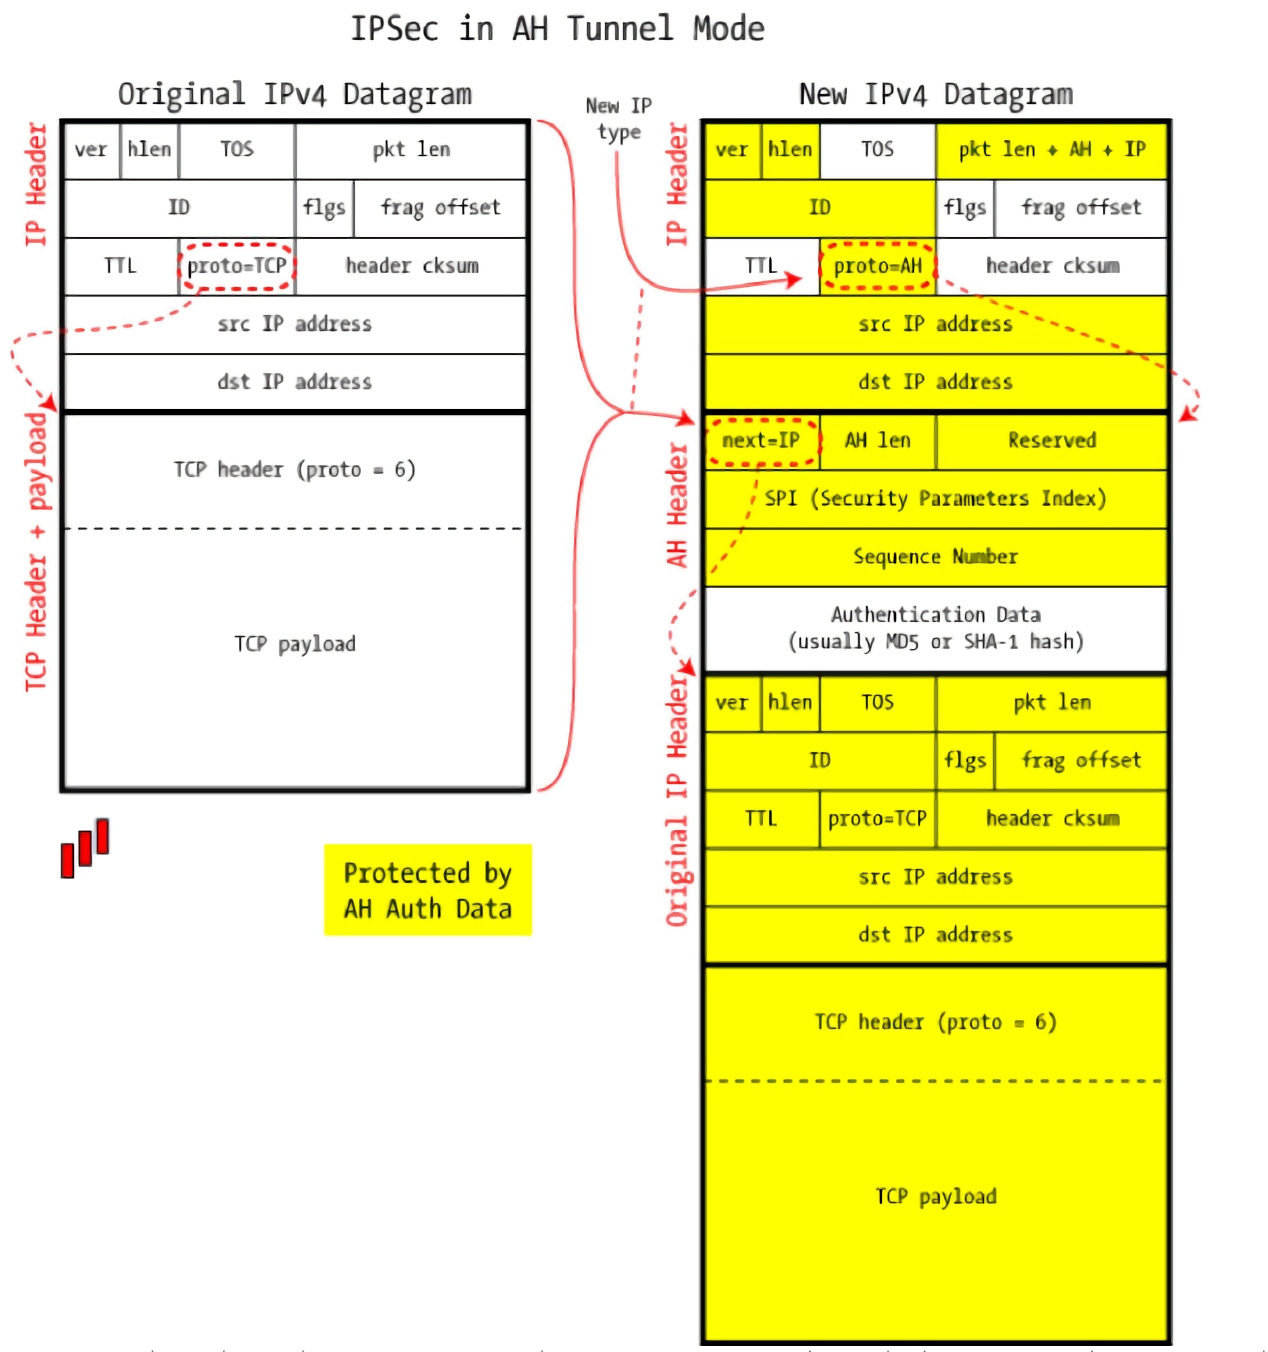
\includegraphics[width=1.0\textwidth]{ah-tunnel.png}
    \caption{隧道模式的AH}
    \label{ah-tunnel}
    \end{figure}

    \begin{figure}[ht!]
    \centering
    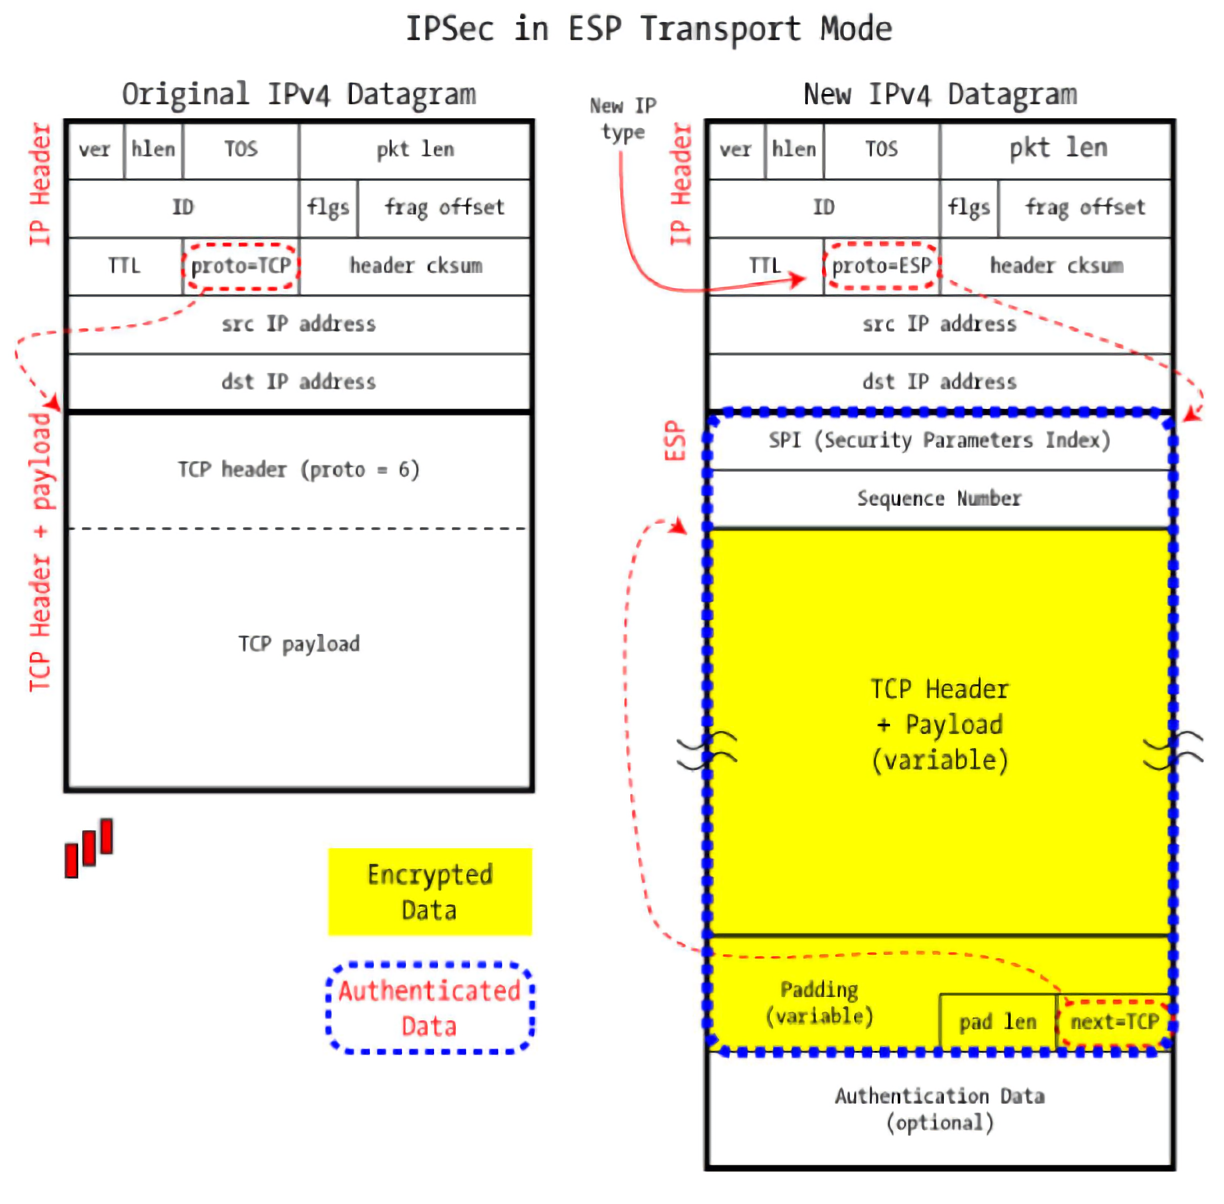
\includegraphics[width=1.0\textwidth]{esp-transport.png}
    \caption{传输模式的ESP}
    \label{esp-transport}
    \end{figure}

    \begin{figure}[ht!]
    \centering
    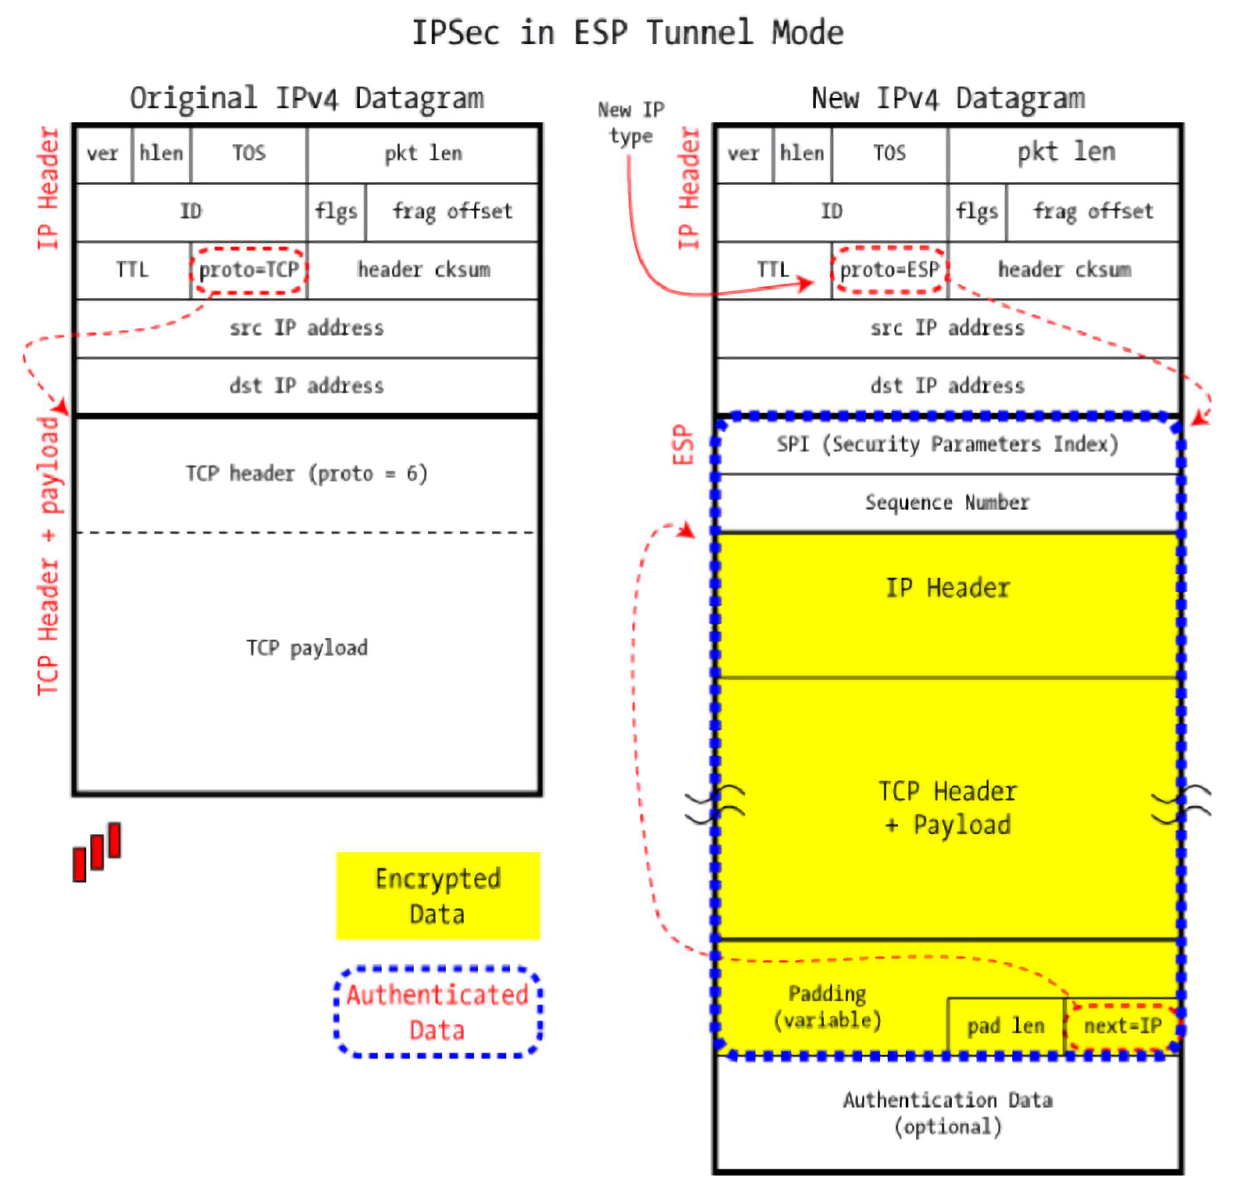
\includegraphics[width=1.0\textwidth]{esp-tunnel.png}
    \caption{隧道模式的ESP}
    \label{esp-tunnel}
    \end{figure}
\clearpage

\subsection{IKE}
    IKE位于应用层 (UDP端口500), 目的是在不安全的互联网上交换密钥,
    使得通信双方能得到一个共有的公共密钥, 用于对称加密或签名.
    此外IKE还需要和SPD, SAD协同工作, 后两者可能请求IKE协商SA.
    \par
    可以采用传输模式端对端地工作, 也可以利用隧道模式在安全网关之间工作.\par

\paragraph{朴素DH的问题} 朴素DH容易受到中间人攻击,
    即欺骗者对 Alice 声称自己是 Bob, 对 Bob 声称自己是 Alice. 解决需要提供Alice和Bob的身份验证.
\subsubsection{第一阶段}
    此阶段协商IKE SA. 有主模式\verb/main mode/和快速模式\verb/aggressive mode/.\par
    双方认证可以有多种方法, 此处以签名认证为例, 摘抄rfc如下\begin{verbatim}
    Phase 1 is where the two ISAKMP peers establish a secure,
       authenticated channel with which to communicate.
5.1 IKE Phase 1 Authenticated With Signatures
    Main Mode with signature authentication is described as follows.
    The first two messages negotiate policy.
    The next two exchange Diffie-Hellman public values
        and ancillary data (e.g.  nonces) necessary for the exchange;
    The last two messages authenticate the Diffie-Hellman Exchange.

        Initiator                          Responder
        -----------                        -----------
        HDR, SA                     -->
                                    <--    HDR, SA
        HDR, KE, Ni                 -->
                                    <--    HDR, KE, Nr
        HDR*, IDii, [ CERT, ] SIG_I -->
                                    <--    HDR*, IDir, [ CERT, ] SIG_R

    Aggressive mode with signatures in conjunction with ISAKMP is described as follows:
    The first two messages negotiate policy, exchange Diffie-Hellman public values
        and ancillary data necessary for the exchange, and identities.
    In addition the second message authenticates the responder.
    The third message authenticates the initiator
    and provides a proof of participation in the exchange.

        Initiator                          Responder
        -----------                        -----------
        HDR, SA, KE, Ni, IDii       -->
                                    <--    HDR, SA, KE, Nr, IDir,
                                                [ CERT, ] SIG_R
        HDR, [ CERT, ] SIG_I        -->

    In both modes, the signed data, SIG_I or SIG_R, is the result of the
    negotiated digital signature algorithm applied to HASH_I or HASH_R
    respectively.

    c.f.
        HDR:    ISAKMP header;  HDR* denotes payloads encrypted.
        SA:     an SA negotiation payload with one or more proposals.
        KE:     public information exchanged in a Diffie-Hellman exchange.
        Nx:     nonce payload;  
        IDx:    identification payload, e.g. IP address
        SIG_x:  necessary info (g^xy, SAx, IDx, Nx etc) signed by x.
\end{verbatim}
\subsubsection{第二阶段}
    协商如IPsec的加密算法, 哈希算法, DH组等等参数.
    使用快速模式\verb/Quick mode/, 需要三次消息交换.

\section{SSL}
\subsection{特点}
    \begin{itemize}
        \item 在IP/TCP参考模型中, SSL / TLS 位于应用层和传输层之间.
        \item SSL工作在 TCP 之上, 不支持 UDP.
    \end{itemize}
\subsection{概念}
    \begin{description}
        \item[会话] 交流双方的一个虚拟的连接关系, 指定了密码算法, 主密钥等等消息.
        \item[连接] 一个通信信道, 通常是一个 TCP 连接.\\
            一个会话可以被多个连接先后使用.
    \end{description}
\subsection{协议}
\subsubsection{SSL记录协议} SSL记录协议定义了SSL传输信息的格式, 是其他SSL协议的基础.\par
    高层数据, 通过SSL, 会经过一下步骤 \begin{enumerate}
        \item 分段, 将高层数据分成小块
        \item 压缩, 这一步是可选的
        \item 计算 MAC 附在数据之后
        \item 使用共享密钥对数据对称加密
        \item 在加密后的数据前添加 SSL 头部
    \end{enumerate}
\subsubsection{握手协议} 握手协议有以下功能\begin{description}
        \item[身份认证] 认证服务器的身份, 并可选地认证客户的身份
        \item[协商密码算法] 包含对称密码算法, MAC 算法以及密钥交换算法
        \item[协商主密钥] 即 master secret, 不过其并不直接用于加密和认证
    \end{description} 之后分为4个阶段\begin{enumerate}
        \item 建立连接, 协商算法
        \item 服务器认证, 服务器发送密钥交换相关消息
        \item 可选的客户端认证, 客户端发送密钥交换相关消息
        \item 完成确认
    \end{enumerate}
\subsection{https应用}
\subsubsection{http的问题}
    \begin{description}
        \item[嗅探监听] 信息不加密
        \item[篡改] 信息没有认证
        \item[伪造服务器] http不验证服务器的可信度
    \end{description}
\subsubsection{https基本概念}
    相对于http, https将消息按照 SSL 加密后再传输, 并且支持通过服务器证书完成的身份验证等.


\section{安全电子邮件}
\subsection{RFC 822}
    定义了最基础的电子邮件传输方式.\par
\paragraph{消息格式} 消息包含信封和内容两个部分, 通过空行隔开. 要求消息是ASCII文本消息.\par
    信封的格式如``关键字: 参数'', 通常有\verb/From/, \verb/To/, \verb/Subject/, \verb/Date/等关键字.
\subsection{MIME}
    针对RFC 822在多媒体传输, 编码等问题, 提出的扩展.\par
    在报头部分增加若干关键字如\verb/Content-Type/, 并且允许多种编码如\verb/base64/.
\subsection{请求响应协议} \begin{description}
        \item[RFC 821] 即SMTP协议, 只处理ASCII数据传输. 没有任何安全措施, 没有密码登陆.
        \item[POP3] 类似SMTP协议, 允许用户名密码登陆.
        \item[IMAP4] 允许有选择地接收邮件等功能.
    \end{description}
\subsection{电子邮件安全问题}
    \begin{description}
        \item[匿名转发] 收件人无法知道真正的发件人
        \item[邮件伪造] 假冒其他人发送邮件
        \item[抵赖] 可伪造的都可以抵赖
        \item[其他] 垃圾邮件和邮件炸弹, 包括邮件病毒等等
    \end{description}
\subsection{S/MIME}
    允许发送 MIME 数据, 提供认证, 加密, 数据完整性和抗抵赖.

    \begin{figure}[ht!]
    \centering
    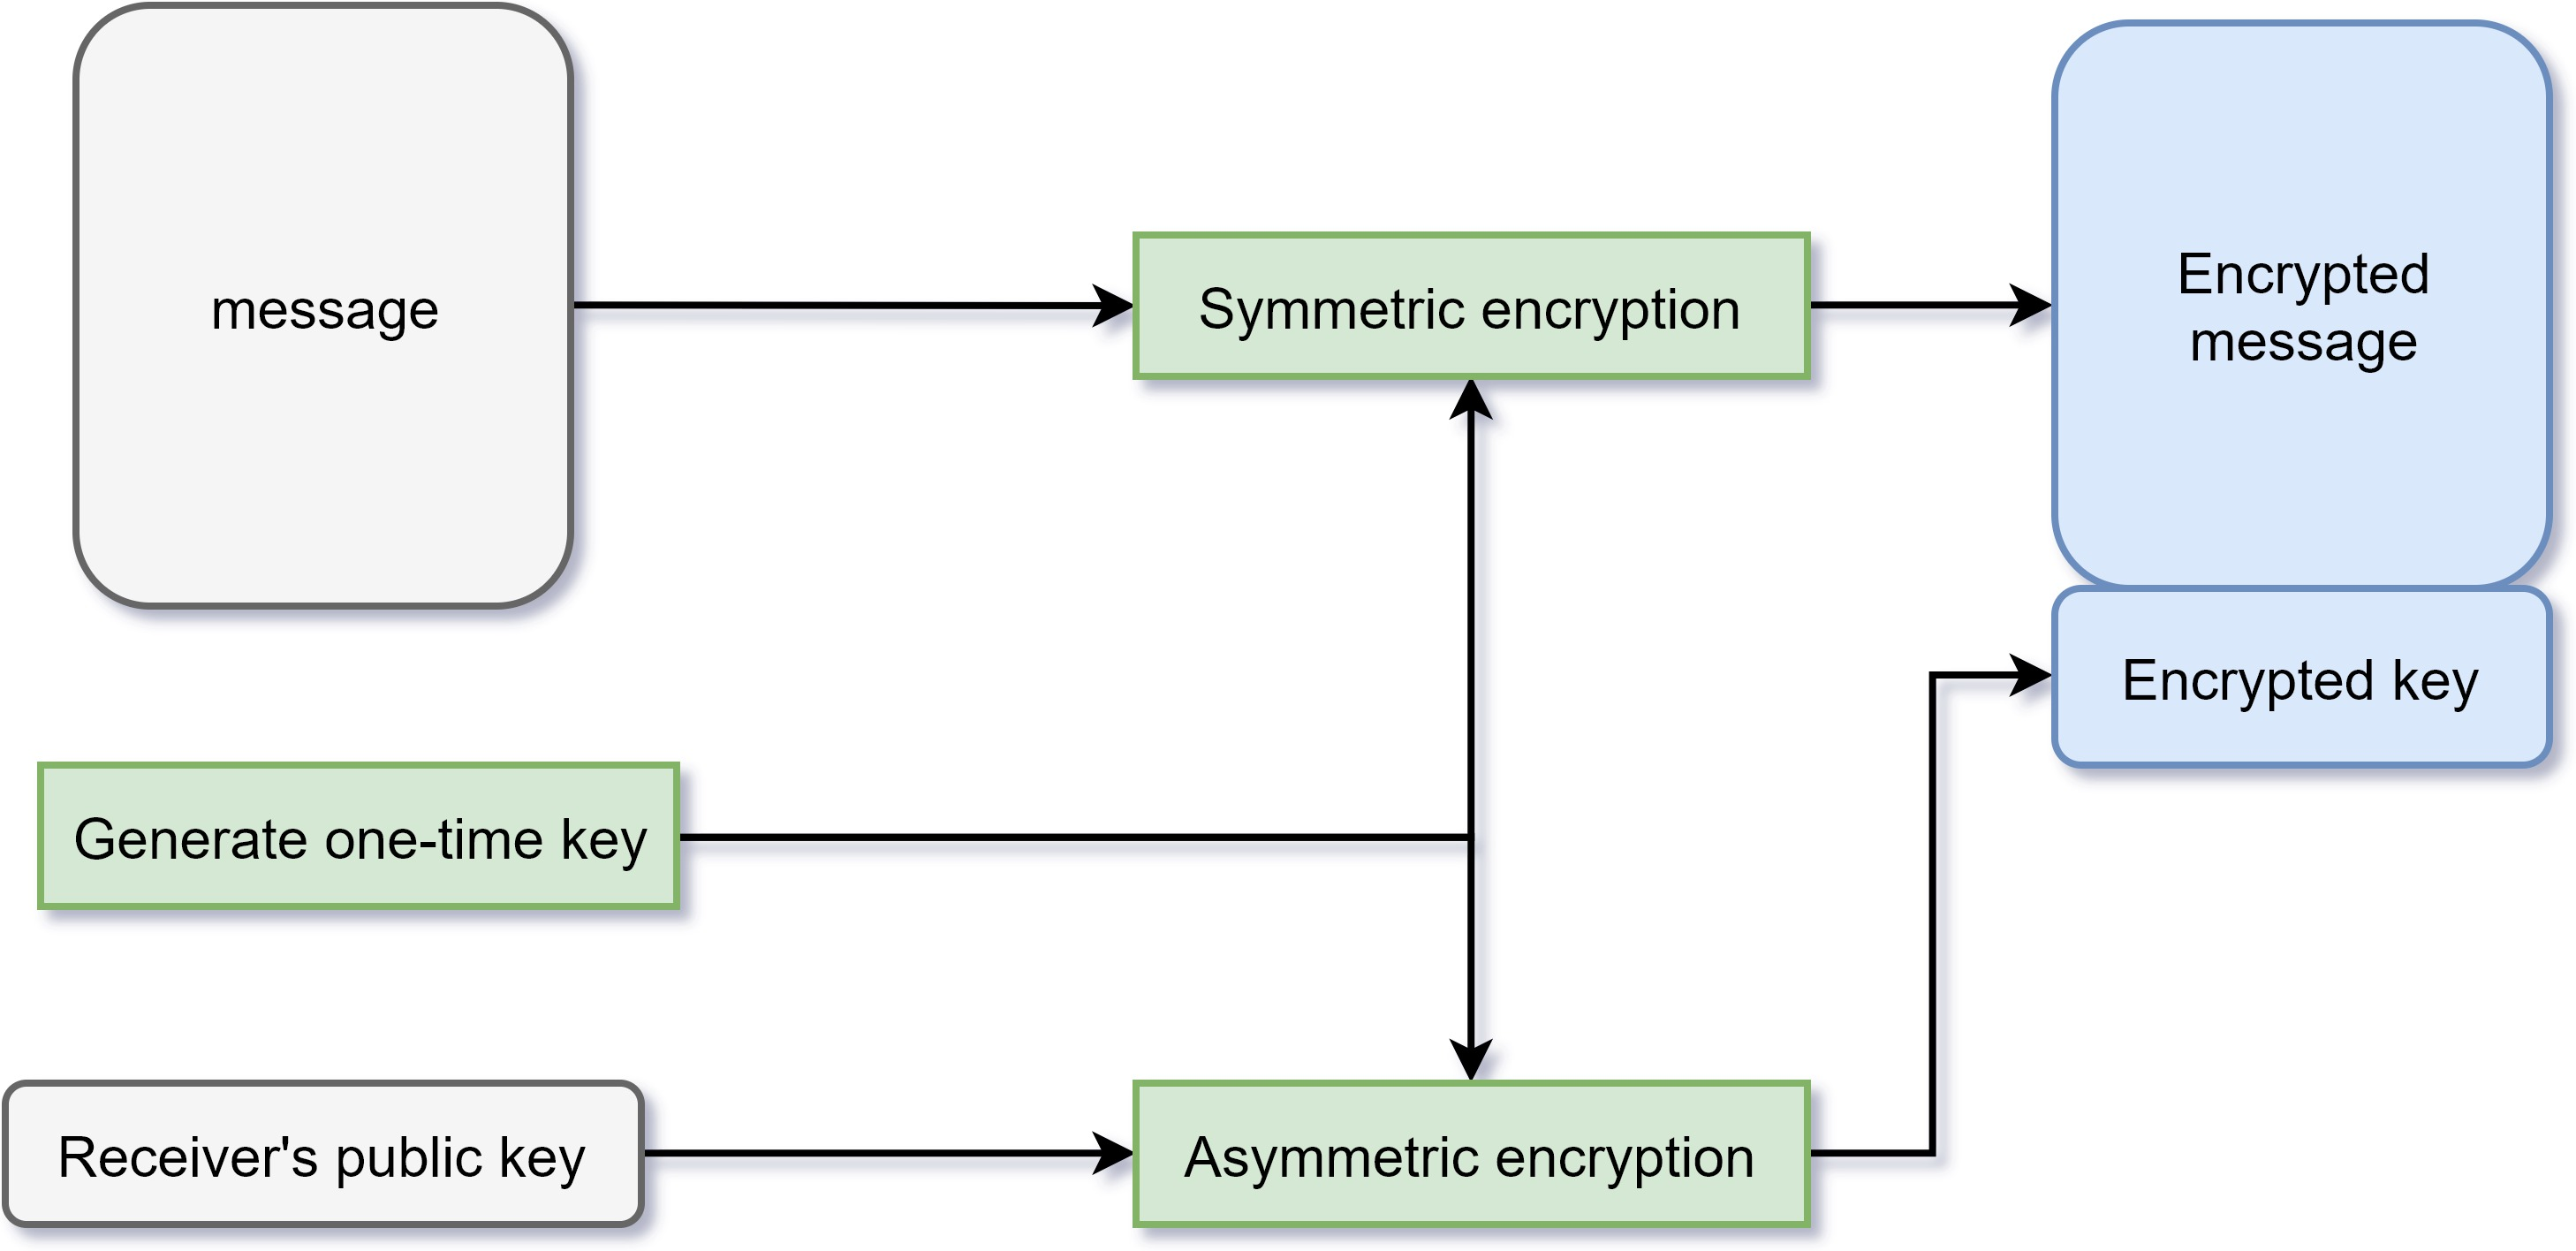
\includegraphics[height=0.5\textheight,width=0.8\textwidth,keepaspectratio]{s-mime-enc.jpg}
    \caption{S/MIME 的加密过程}
    \label{s-mime-enc}
    \end{figure}

    \begin{figure}[ht!]
    \centering
    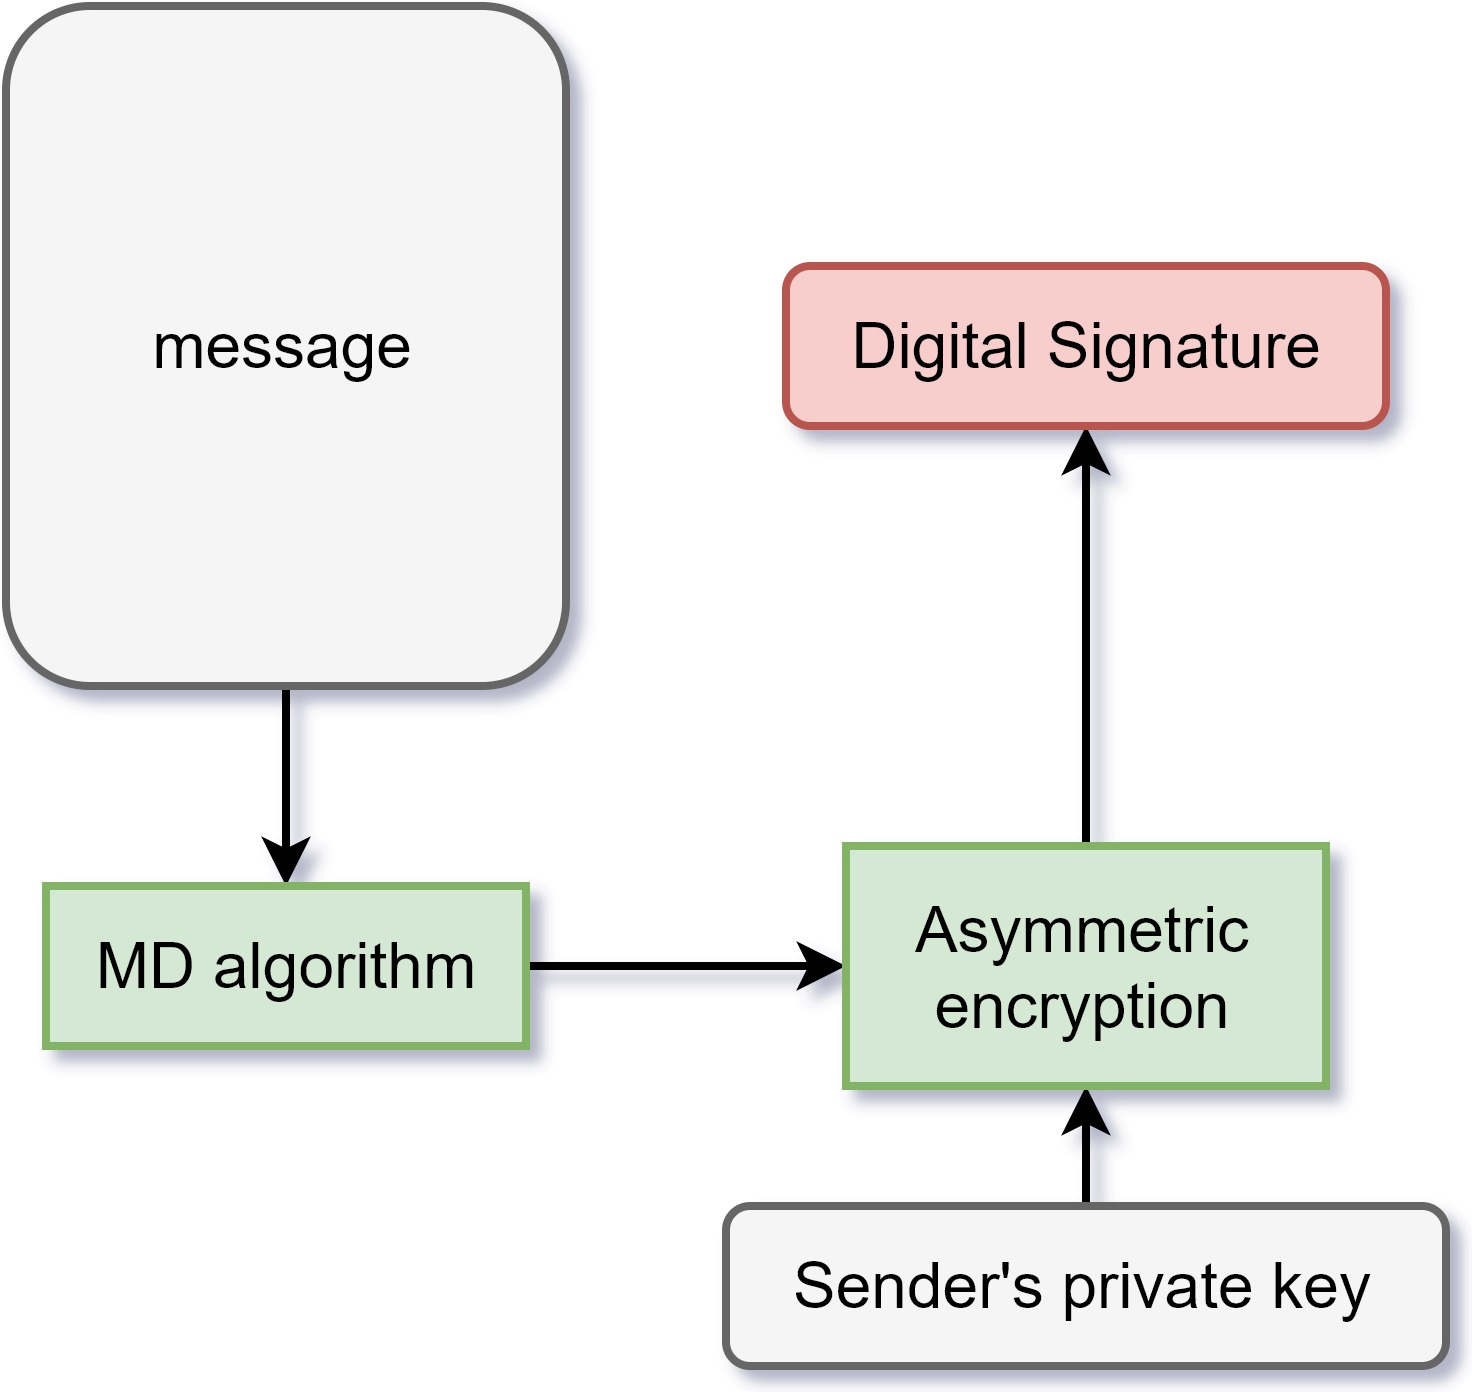
\includegraphics[height=0.4\textheight,width=0.8\textwidth,keepaspectratio]{s-mime-ds.jpg}
    \caption{S/MIME 的数字签名}
    \label{s-mime-ds}
    \end{figure}

    S/MIME支持透明签名, 即对空消息进行数字签名后发送.

\section{安全电子商务}
\subsection{安全需求和安全问题}
    \begin{itemize}
        \item 资金流动的保密性. 防止第三方截获交易信息
        \item 支付结算数据的完整性. 防止篡改数据
        \item 支付双方身份认证.
        \item 抗抵赖
        \item 效率等
    \end{itemize}
    SET协议基于信用卡, 完成了\begin{itemize}
        \item 私密性
        \item 保密性
        \item 完整性
        \item 抗抵赖
    \end{itemize}
\subsection{SET协议}
\subsubsection{参与方}
    \begin{description}
        \item[持卡人]   意即消费者
        \item[商家]     事先和收款行建立信任关系
        \item[发卡行]   消费者持卡的银行
        \item[收款行]   代替商家与多个发卡行联系, 验证持卡人信息的有效性
        \item[证书权威] 可信的第三方, 为持卡人, 商家, 收款行提供证书
        \item[支付网关] 收款行控制, 处理商家的支付报文.
    \end{description}
\subsubsection{流程}
\paragraph{双签名} 交易中有两种信息, 订单相关和支付相关的.
    只有商家才能看到订单相关的, 只有银行才能看到支付相关的.
    然而需要对两种信息都签名, 并允许商家和银行验证两种信息的签名.\par
    双签名的计算即如\[
        \mathrm{Dual\,Signature} = E_{\mathrm{KR}_C} [H(\mathrm{PIMD} \;\|\; \mathrm{OIMD})] \]
\paragraph{购买请求}
    如图
    \begin{figure}[ht!]
    \centering
    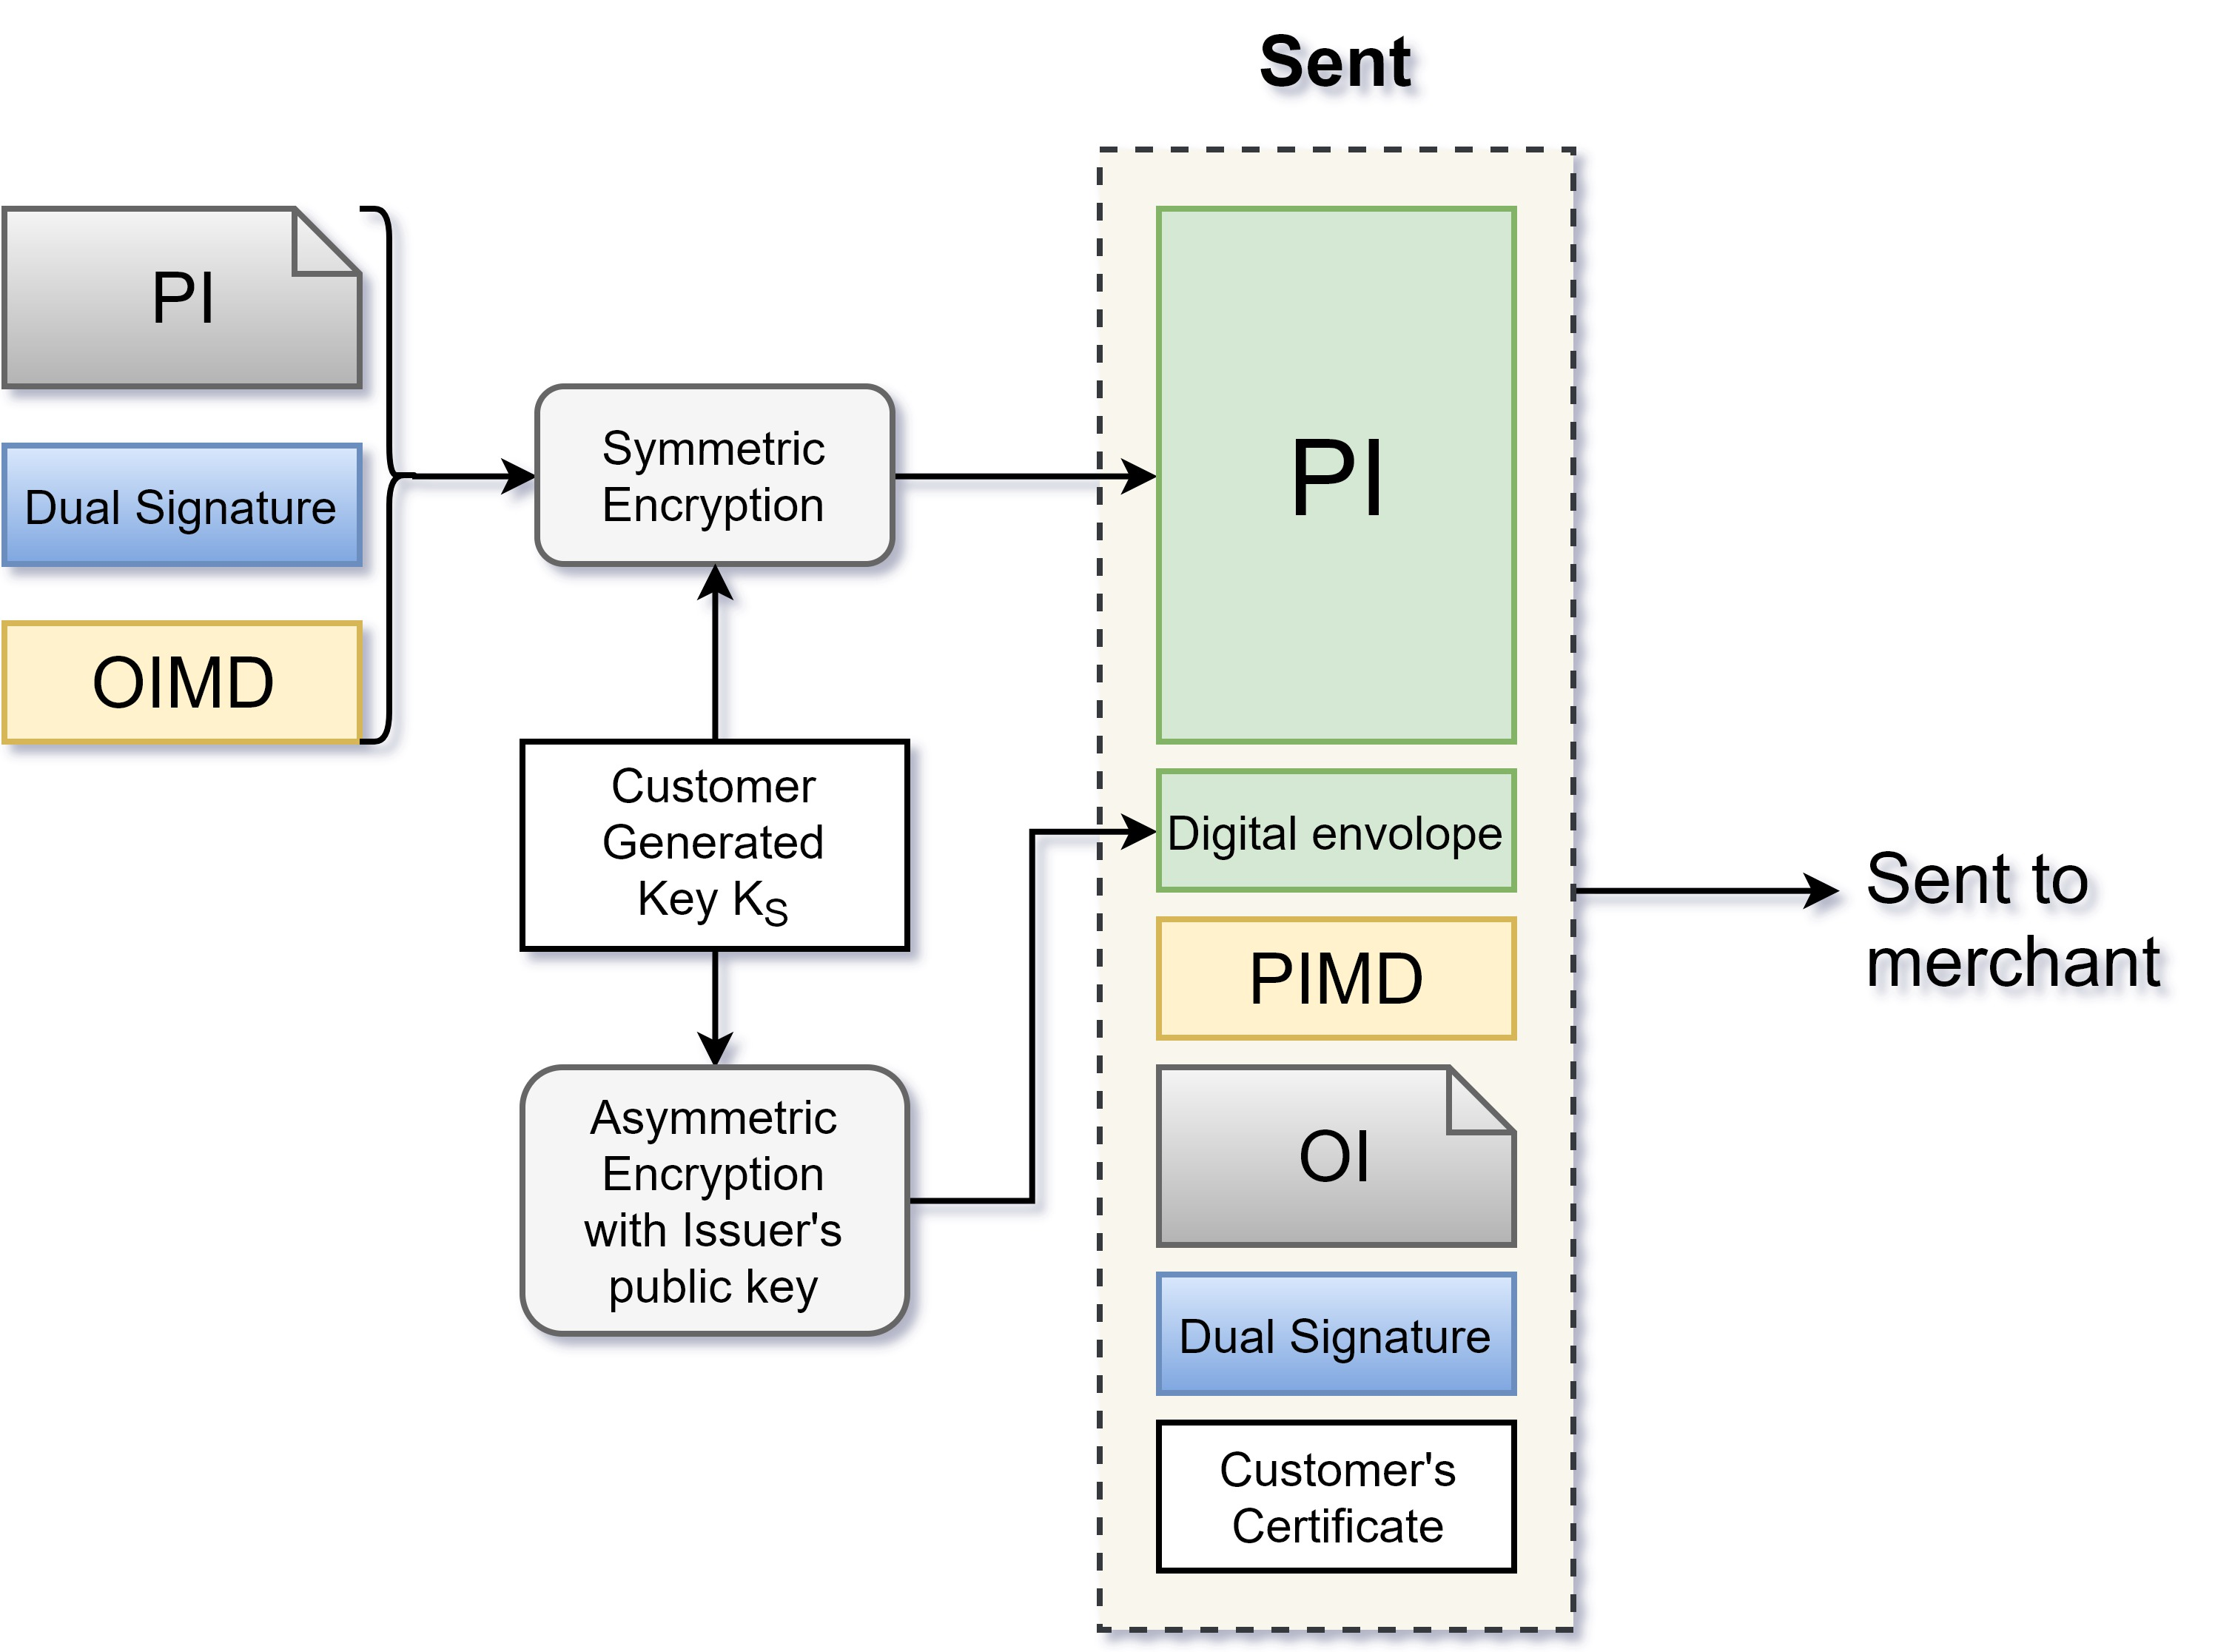
\includegraphics[width=\textwidth]{set-1.jpg}
    \caption{购买请求, Customer端}
    \label{set-1}
    \end{figure}
    \begin{figure}[ht!]
    \centering
    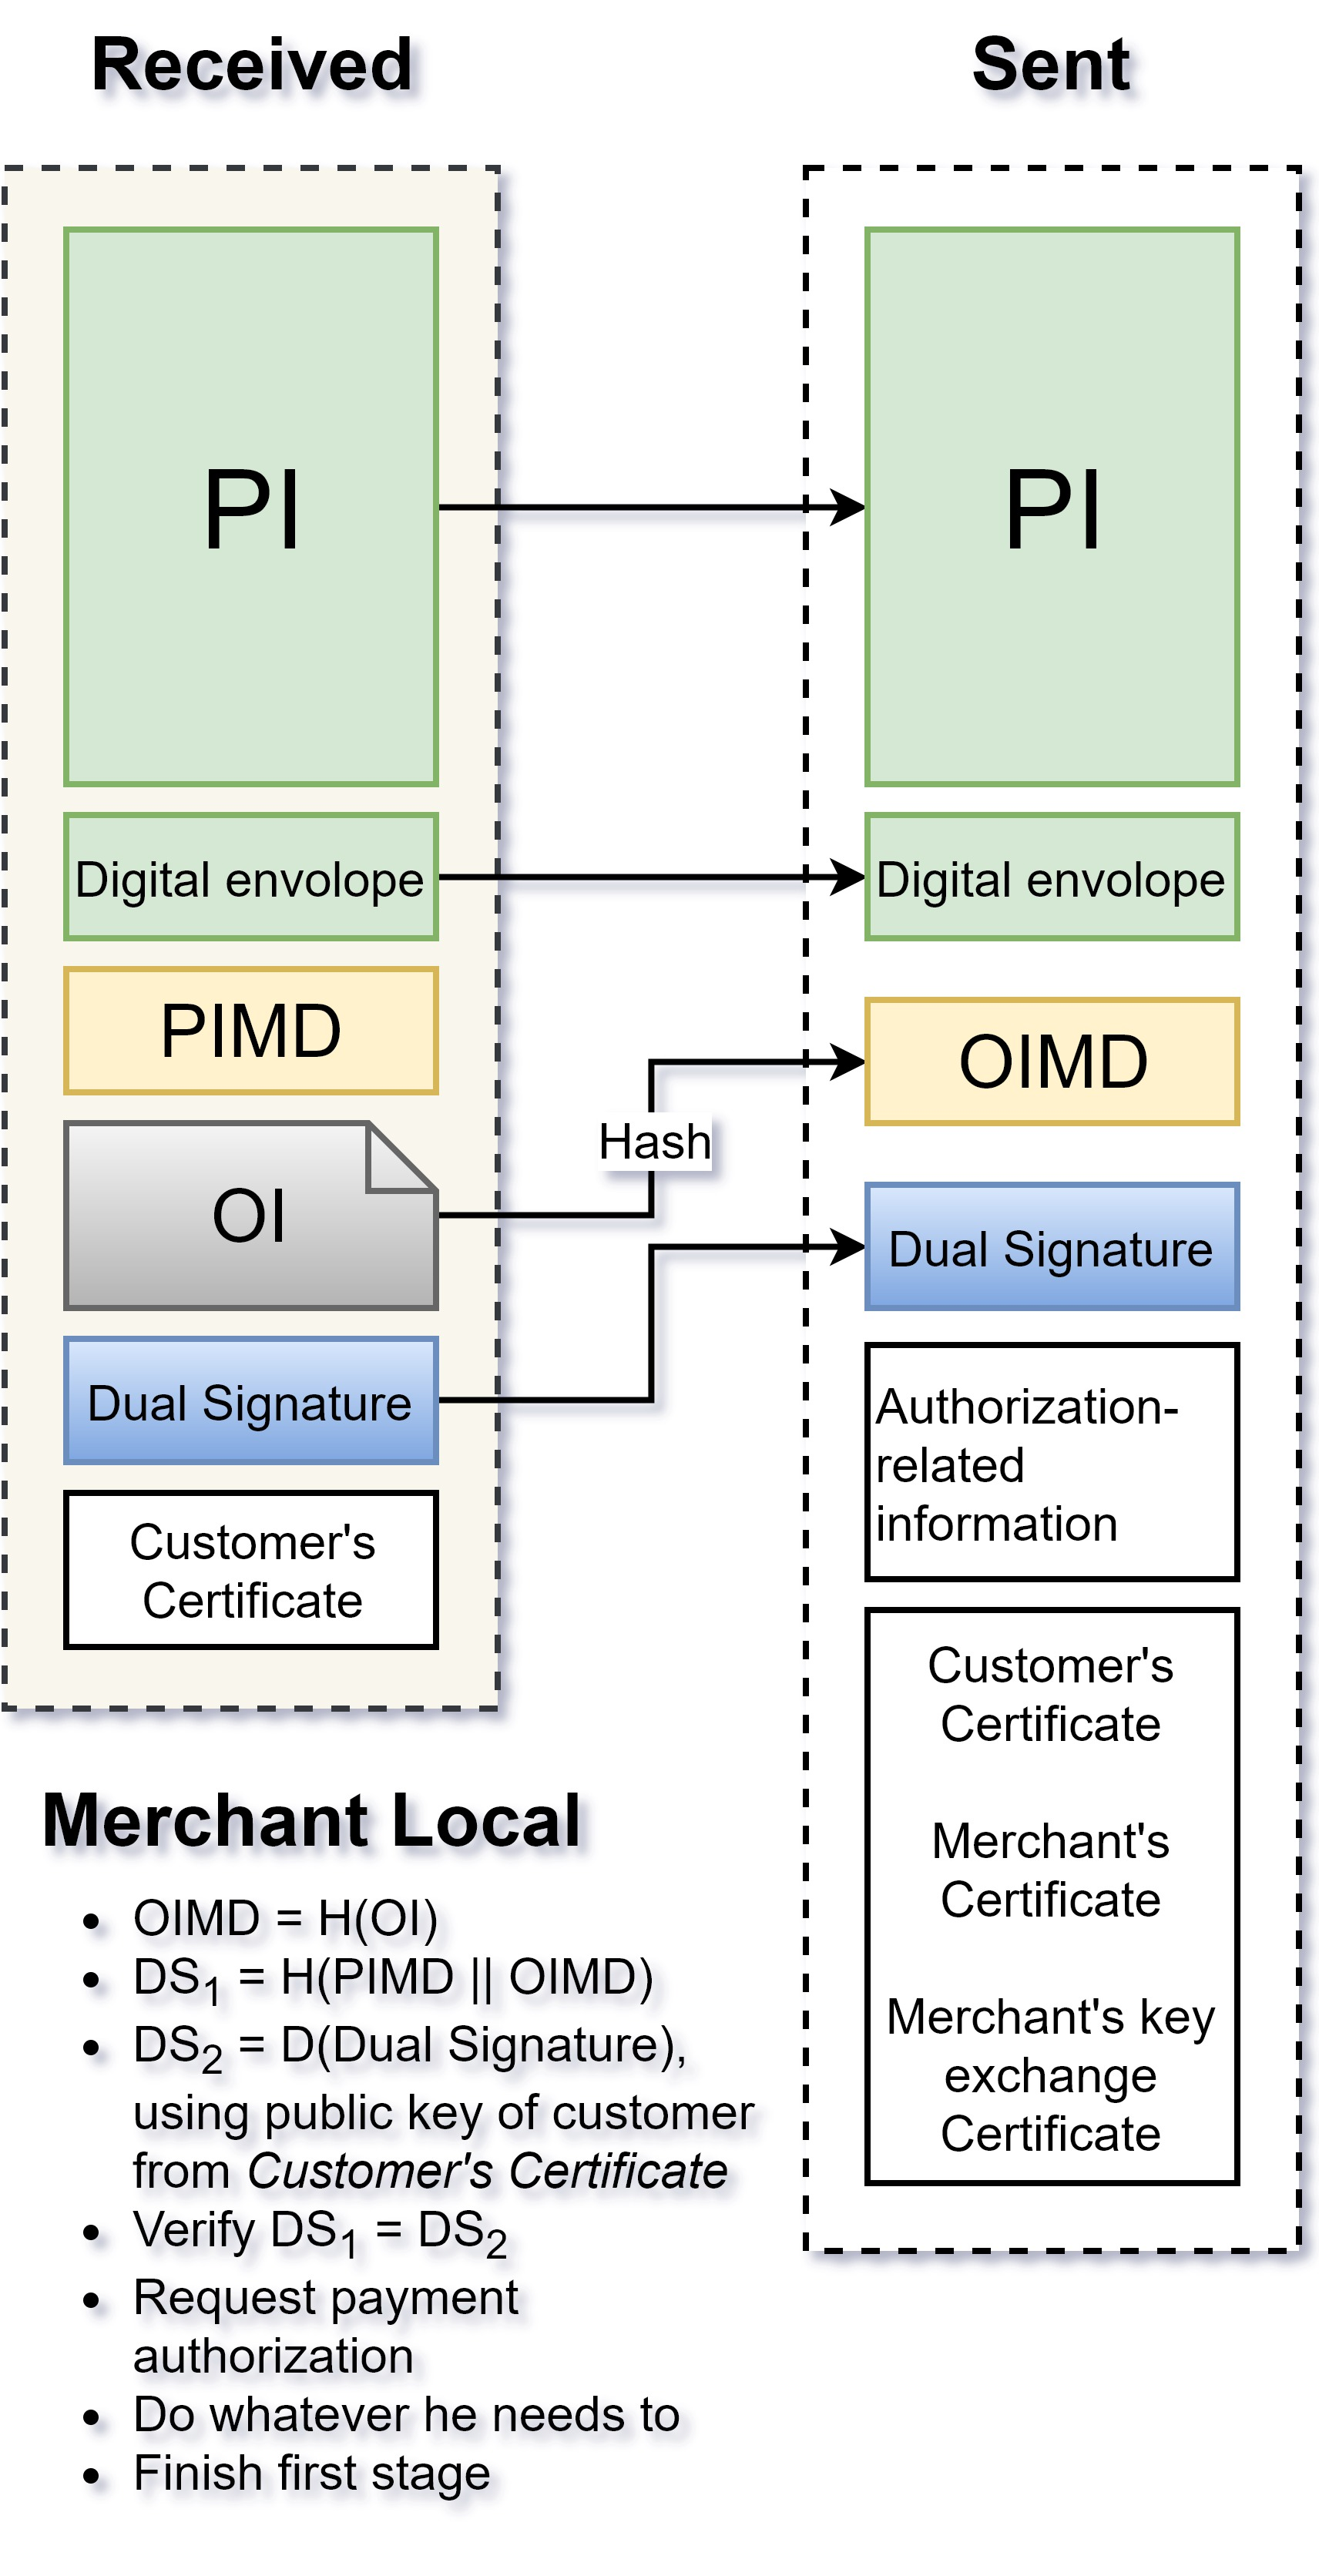
\includegraphics[height=\textheight, width=\textwidth, keepaspectratio]{set-2.jpg}
    \caption{购买请求, Merchant端}
    \label{set-2}
    \end{figure}

\clearpage
\paragraph{支付授权}
    \begin{enumerate}
        \item Merchant 给 Acquirer 发送支付授权请求
        \item Acquirer 确认授权, 给 Issuer 发送划款请求
    \end{enumerate}
\paragraph{支付获取}
    完成转账业务

\section{入侵技术}
\subsection{入侵检测}
\paragraph{审计记录} 包含用户活动记录, 用于检测用户的行为.
\subsubsection{基于统计的入侵检测}
    能够防范假冒者, 但是不能防范合法用户.\par
    \begin{description}
        \item[阈值检测] 检测一段时间内某用户产生的各种事件.
            如果, 事件发生次数超过其阈值, 则认为可能存在入侵.\\
            本身是很粗糙的, 容易误判.
        \item[轮廓检测] 为每个用户建立一个行为轮廓, 学习其行为模式,
            检测用户行为模式的异常变化.
    \end{description}
\subsubsection{基于规则的入侵检测}
    基本原理是检测系统中发生的事件,
    运用先定的规则集确定某一个活动模式是否可疑.
    其中先定的规则集是专家系统定义的.
\subsubsection{蜜罐}
    创建一个正常用户不会访问的蜜罐系统,
    引诱攻击者攻击这个没有有用信息的蜜罐系统.\par
    任何对于蜜罐的访问都是可疑的.
\subsection{软件入侵}
    \begin{table}[ht!]
        \centering
    \begin{tabularx}{\textwidth}{|C|C|C|C|}
        \Topline
                &           病毒 &              蠕虫 &          木马 \\
        \Midline
        宿主    &           需要 &            不需要 &          需要 \\
        \Midline
        表现形式 &          不以文件 &      独立的文件 &    伪装成其他文件\\
        \Midline
        传播方式 &  依赖宿主    &           自主传播 &          依靠用户主动传播\\
        \Midline
        危害 &      破坏数据/系统完整性 &   侵占资源 &      留下后门 \\
        \Midline
        传播速度 &          快 &            很快    &       慢 (不能自我复制)\\
        \Bottomline
    \end{tabularx}
        \caption{各种恶意软件的特点}
    \end{table}
\subsubsection{后门}
    软件中秘密入口, 可以绕过通常步骤获得权限.
    控制方式包含本地权限提升, 远程执行程序等.
\subsubsection{逻辑炸弹}
    当特定事件发生时, 在被执行制造破坏的代码.
\subsubsection{特洛伊木马}
    伪装成正常程序, 欺骗安装和运行, 使攻击者能获得权限.
    类似后门, 但重点在伪装成正常程序的欺骗性.
\subsubsection{Zombie}
    秘密接管Internet上的计算机, 利用这些计算机发送攻击 (常是DoS).
\subsubsection{病毒}
    一段可以通过修改自身, 修改其他程序的 程序片段.
\subsubsection{蠕虫}
    完整独立的计算机程序, 能够自我复制, 并通过计算机网络传播.

%\pagebreak
%\appendix
%
%\section{实验 IDS}
%\subsection{检测技术}
%\subsubsection{基于异常}
%    学习正常流量的特征, 只允许满足特征的包.\par
%    较高误报率, 较低漏报率.
%\subsubsection{基于特征}
%    学习异常流量的特征, 不允许满足特征的包.\par
%    较高漏报率, 较低误报率.
%\subsection{常见攻击}
%\subsubsection{DoS/DDoS攻击}
%    不停访问目标资源, 使得目标资源耗尽.
%\subsubsection{DNS放大攻击}
%    DNS特点: 回复包比请求包大很多. 方法是伪造发送者, 类似DoS.
%\subsection{实验命令}
%\paragraph{离线模式}
%\begin{verbatim} suricate -c CONFIG_PATH -l LOG_PATH -r DETECT_OUTPUT_PATH \end{verbatim}
%
%\section{实验 Packet Tracer}
%\subsection{设备使用}
%\subsubsection{交换机} 位于链路层. 为端到端通信提供不被干扰的链路.
%\subsubsection{路由器} 位于网路层. cisco IOS 四种模式包含.
%    usr mode        router>
%    privlge mode    router#
%    conf mode       router(config)#
%    spec conf mode
%     enable : usr -> privlge
%     disable: privlge -> usr
%     configure terminal:     privlge -> conf
%   routing tbl: <dest, mask, nexthop>
%   interface connections:
%       PC: 1 2 send; 3 6 recv;
%       switch: 1 2 recv; 3 6 send;
%       straight-through:   PC - switch
%       cross-over:         PC - PC, switch - switch
%   switch 2960: both straight-through / cross-over are ok to use


\end{document}

